\documentclass[8pt]{beamer}

%%%%%%%%%%%%
% PACKAGES %
%%%%%%%%%%%%

% kek 
\usepackage[T1]{fontenc} % Use 8-bit encoding that has 256 glyphs
\usepackage[utf8]{inputenc} % For Spanish characters
\usepackage[english]{babel} % USEnglish localization
% =========== General Formatting =============
\usepackage{microtype} % Slightly tweak font spacing for aesthetics
\usepackage{fancyhdr} % Allows for nice header and footer
\usepackage{appendix} % Enables appendices
\usepackage{enumerate} % Custom numerate, useful for i,ii,iii... I,II,III...
% \usepackage{hyperref} % For hyperlinks in the PDF
\usepackage{extramarks} % 
\usepackage{fontawesome} % For web icons

% =============== Math ===============
\usepackage{amsmath} % Standard math packages
\usepackage{amsthm} % Math Theorems
\usepackage{amssymb} % Math Symbols
\usepackage{amsfonts} % Math Fonts
\usepackage{mathtools} % Extra math tools such as PairedDelimiter
\usepackage{upgreek} % Nice sigma => \upsigma
\usepackage{array} % Enables array features
\usepackage{siunitx} % For SI Unit easy formatting
\usepackage{dsfont} % For math. indicators

% =============== Figures ===============
\usepackage{float} % Float features
\usepackage{wrapfig} % Al­lows fig­ures or ta­bles to have text wrapped around them
\usepackage{tikz} % Diagram and figure creation and rendering
% =============== Tables ===============
\usepackage{booktabs} % Horizontal rules in tables
\usepackage{float} % Required for tables and figures in the multi
\usepackage{multirow} % Combined rows in tables
\usepackage{multicol} % Combined columns in tables
\usepackage{colortbl} % Color cells
%\usepackage{longtable} % Tables than span multipages

% =============== Bibliography ==========
\usepackage{natbib} % Lots of useful versions of \cite

% % =============== Listings ============
\usepackage{listings} % Main package for inserting code
\usepackage[scaled]{beramono} % For using the beramono font
% % =============== Algorithms ===============
\usepackage[linesnumbered,lined,boxed,commentsnumbered]{algorithm2e} % Allows for algorithm description
\usepackage[noend]{algpseudocode}
% =============== Other ===============
\usepackage{datetime} % Date-Time formatting
\usepackage{ulem} % For strikethrough text \st{}
\usepackage{textcomp} %Text Com­pan­ion fonts

\usepackage{pdfpages} % Insert pdfs
\usepackage{lipsum} % Used for inserting dummy 'Lorem ipsum' text into the template
% \usepackage[space]{grffile} % insert files with spaces
\usepackage{pdflscape} % Individual horizontal pages
\usepackage[many]{tcolorbox} % Color boxes for comment
%\usepackage{xargs} % Expanded arguments features
%\usepackage{fix-cm} % Computer-Modern at arbitrarysizes
%\usepackage{eurosym} % Eurosymbol

% Thick strike out
\newcommand{\cancelled}[1]{%
    \renewcommand{\ULthickness}{3pt}%
       \sout{#1}%
    \renewcommand{\ULthickness}{.4pt}% Resetting to ulem default
}

\newcommand{\done}[1]{\sout{#1}}

% derivatives
\newcommand{\dderiv}[2]{\frac{\mathrm{d}}{\mathrm{d}#2} (#1)}

% partial derivatives
\newcommand{\pderiv}[2]{\frac{\partial #1}{\partial #2}}
\newcommand*{\pd}[3][]{\ensuremath{\frac{\partial^{#1} #2}{\partial #3}}}

% Integral dx
\newcommand{\dx}{\mathrm{d}x}

% Evaluation operator
\newcommand*{\at}[2]{\Big|_{#1}^{#2}}

% Probability macros
% Variance
\newcommand{\Var}{\mathrm{Var}}
% Covariance
\newcommand{\Cov}{\mathrm{Cov}}
% Bias
\newcommand{\Bias}{\mathrm{Bias}}
% Probability
\newcommand*{\prob}[1]{\ensuremath{\mathbb{P}\left[#1\right]}}
\newcommand*{\expectation}[1]{\ensuremath{\mathbb{E}\left[#1\right]}}
\newcommand*{\variance}[1]{\ensuremath{\mathbb{V}\left[#1\right]}}
% Indicator function of an event
\newcommand*{\ind}[1]{\ensuremath{\mathds{I}_{\left[#1\right]}}}

% Optimization macros
\DeclareMathOperator{\dom}{Dom}
\DeclareMathOperator{\diag}{Diag}
\DeclareMathOperator{\prox}{prox}
\DeclareMathOperator*{\proj}{Proj}
\DeclareMathOperator*{\sign}{sign}
\DeclareMathOperator*{\argmax}{argmax}
\DeclareMathOperator*{\argmin}{argmin}

\newcommand*{\pdef}{\ensuremath{\mathbb{S}_{++}}}
\newcommand*{\psdef}{\ensuremath{\mathbb{S}_{+}}}

%% \mathbb symbols
\DeclareMathOperator{\E}{\mathbb{E}}
\DeclareMathOperator{\A}{\mathbb{A}}
\DeclareMathOperator{\B}{\mathbb{B}}
\DeclareMathOperator{\R}{\mathbb{R}}
\DeclareMathOperator{\C}{\mathbb{C}}
\DeclareMathOperator{\X}{\mathbb{X}}
\DeclareMathOperator{\N}{\mathbb{N}}
\DeclareMathOperator{\Q}{\mathbb{Q}}
\DeclareMathOperator{\V}{\mathbb{V}}

%% \mathcal symbols
\DeclareMathOperator{\RR}{\mathcal{R}}
\DeclareMathOperator{\PP}{\mathcal{P}}
\DeclareMathOperator{\NN}{\mathcal{N}}
\DeclareMathOperator{\CC}{\mathcal{C}}
\DeclareMathOperator{\FF}{\mathcal{F}}
\DeclareMathOperator{\YY}{\mathcal{Y}}
\DeclareMathOperator{\XX}{\mathcal{X}}
\DeclareMathOperator{\LL}{\mathcal{L}}

%% \tilde symbols
\newcommand{\tbeta}{\tilde\beta}
\newcommand{\tgamma}{\tilde\gamma}

%% \hat symbols
\newcommand{\hbeta}{\hat{\beta}}
\newcommand{\hgamma}{\hat{\gamma}}
\newcommand{\hxi}{\hat{\xi}}

% limit arrow "goes to"
\newcommand{\goto}{\rightarrow}

% text above math symbol
\newcommand{\textabove}[2]{\mathrel{\overset{\makebox[0pt]{\mbox{\normalfont\tiny #1}}}{#2}}}

% Big O
\newcommand{\bigo}{{\mathcal O}}

% 1/2
\newcommand{\half}{\frac{1}{2}}
% 1/2
\newcommand{\halfof}[1]{\frac{#1}{2}}

% Real numbers
\newcommand\reals{{{\rm l} \kern -.15em {\rm R} }}

% Complex numbers
\newcommand\complex{{\raisebox{.043ex}{\rule{0.07em}{1.56ex}} \hskip -.35em {\rm C}}}

% Matrix functions
\DeclareMathOperator{\trace}{Tr}

% matrix environment for vectors or matrices where elements are centered
\newenvironment{mat}{\left[\begin{array}{ccccccccccccccc}}{\end{array}\right]}
\newcommand\bcm{\begin{mat}}
\newcommand\ecm{\end{mat}}

% matrix environment for vectors or matrices where elements are right justified
\newenvironment{rmat}{\left[\begin{array}{rrrrrrrrrrrrr}}{\end{array}\right]}
\newcommand\brm{\begin{rmat}}
\newcommand\erm{\end{rmat}}

% for left brace and a set of choices
\newenvironment{choices}{\left\{ \begin{array}{ll}}{\end{array}\right.}
\newcommand\when{&\text{if~}}
\newcommand\otherwise{&\text{otherwise}}
% sample usage:
%  \delta_{ij} = \begin{choices} 1 \when i=j, \\ 0 \otherwise \end{choices}

% For equations: first argument is a label, second is the equation 
\newcommand{\eql}[2]{\begin{equation}\label{eq:#1}\begin{split}#2\end{split}\end{equation}}
% Or just the equation 
\newcommand{\eq}[1]{\begin{equation}\begin{split}#1\end{split}\end{equation}}

% some useful macros for finite difference methods:
\newcommand\unp{U^{n+1}}
\newcommand\unm{U^{n-1}}
\newcommand\un{U^{n}}

% paired parenthesis
\DeclarePairedDelimiter\pa{(}{)}%
\DeclarePairedDelimiter\bra{[}{]}%
\DeclarePairedDelimiter\curly{\{}{\}}%
\DeclarePairedDelimiter\abs{\lvert}{\rvert}%
\DeclarePairedDelimiter\norm{\lVert}{\rVert}%
\DeclarePairedDelimiter\floor{\lfloor}{\rfloor}%
\DeclarePairedDelimiter\ceil{\lceil}{\rceil}%

% colorful box (for putting around equality signs etc)
\newtcbox{\mywboxtext}[1]{on line,colback=white,colframe=#1,size=fbox,arc=3pt,boxrule=0.8pt}
\newcommand{\boxaround}[2]{\mywboxtext{#2}{$#1$}}





% \usetheme[progressbar=frametitle]{metropolis}
\usepackage{appendixnumberbeamer}
\addbibresource{../bibliography.bib}

% PRESETS OF PACKAGES AND MATH %

\usepackage{xspace}
\usepackage{caption}
\usepackage{subcaption}
\usepackage{lmodern}
\newcommand{\themename}{\textbf{\textsc{metropolis}}\xspace}
\newcommand{\ouralgo}{\ensuremath{\mathcal{MSR}3}}
\title{PhD Defense}
\date{\today}
\author{Aleksei Sholokhov}
%\titlegraphic{
\includegraphics[width=0.5\textwidth]{Figures/UW_amath.pdf}\hspace{3em}
\includegraphics[height=1cm]{Figures/IHME_Logo.jpg}}

\AtBeginSection[]{
  \begin{frame}
  \vfill
  \centering
  \begin{beamercolorbox}[sep=8pt,center,shadow=true,rounded=true]{title}
    \usebeamerfont{title}\insertsectionhead\par%
  \end{beamercolorbox}
  \vfill
  \end{frame}
}

\begin{document}

\maketitle

%\section{Introduction}
\begin{frame}{Plan of the Defense}
Show topics and published papers. Mention covid
\end{frame}

\section{$\mathcal{MSR}3$ -- Sparse Relaxed Regularized Regression for Linear Mixed-Effect Models}

\begin{frame}{Linear Mixed-Effect (LME) Models}

	Dataset: $m$ groups $(X_i, Z_i, y_i),\quad i = 1, \dots m$, each has $n_i$ observations
	\begin{itemize}
		\item 	$X_i \in \R^{n_i \times p}$ -- group $i$ design matrix for fixed features
		\item 	$Z_i \in \R^{n_i \times q}$ -- group $i$ design matrix for random features
		\item 	$y_i \in \R^{n_i}$ -- group $i$ observations  
		\item   $u_i \in \R^q$ -- random effects
		\item   $\Gamma \in \R^{q \times q}$ -- covariance matrix of random effects, often $\Gamma = \diag{(\gamma)}$
		\item   $\Lambda_i \in R^{n_i \times n_i}$ -- covariance matrix for observation noise
	\end{itemize}
	

	\begin{columns}[T,onlytextwidth]
	
    \column{0.5\textwidth}
    \vspace{3em}
    Model:
	 	\[
   		\begin{split}
   			y_i & = X_i\beta + {\color{red}Z_i u_i} + \varepsilon_i \\
   			 \varepsilon_i & \sim \NN(0, \Lambda_i) \\
   			{\color{red} u_i} & {\color{red}\sim \NN(0, \Gamma)}
   		\end{split}
   		\]
   		   	
	Unknowns: $\beta$, $u_i$, $\gamma$, sometimes $\Lambda_i$.
	
    \column{0.5\textwidth}
    	\centering  
   	\begin{figure}
   		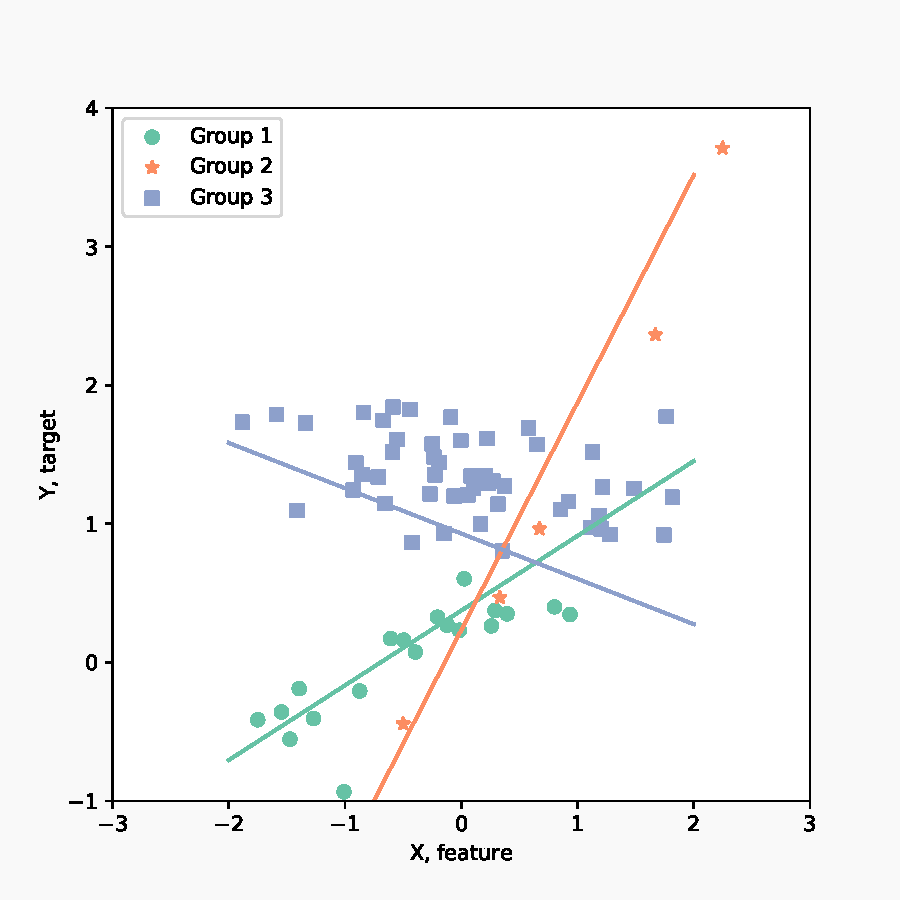
\includegraphics[width=0.9\textwidth]{Figures/lme_example_random_prediction}
   	\end{figure}
   	   		

   	
  \end{columns}
\end{frame}

\begin{frame}{Mixed-Effect Models}
Mixed-effect models
\begin{itemize}
	\item Used for analyzing \textbf{combined data} across a range of \textbf{groups}.
	\item Use covariates to separate the \textbf{population variability} from the \textbf{group variability}.
	\item \textbf{Borrow strength} across groups to estimate key statistics. % when data within units are sparse or highly variable.
\end{itemize}

\begin{figure}
	\centering
	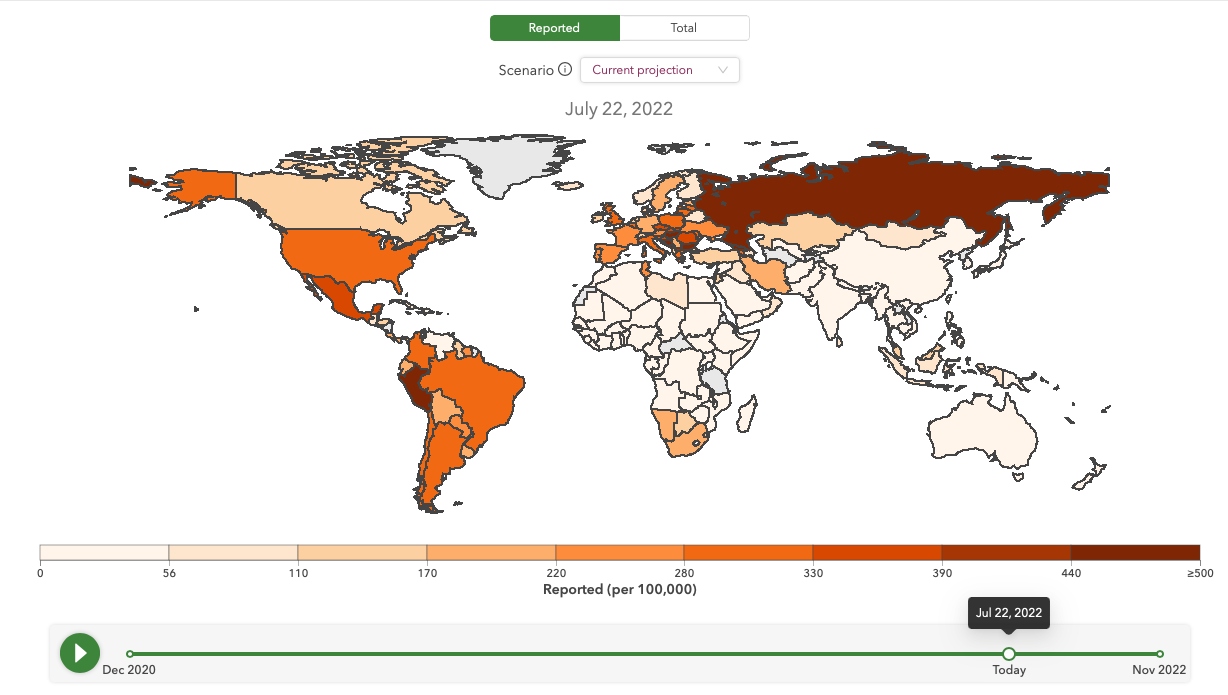
\includegraphics[width=0.8\textwidth]{Figures/ihme_predictions.png}\footnote{Picture is taken from \href{covid19.healthdata.org}{covid19.healthdata.org} }
\end{figure}

\end{frame}

%\begin{frame}{Notation}
%	\eq{
%   		y_i & = X_i\beta + Z_iu_i + \varepsilon_i \quad i = 1\dots m \\
%   		\varepsilon_i & \sim \NN(0, \Lambda_i) \\
%   		u_i & \sim \NN(0, \Gamma)
%   	}   	
%   	
%   	\begin{itemize}
%   		\item $p$ -- number of fixed features, $q$ -- number of random effects.
%   		\item $\beta \in \R^p$ -- fixed effects, or mean effects
%   		\item $u_i \in \R^q$ -- random effects
%   		\item $\Gamma \in \R^{q \times q}$ -- covariance matrix of random effects, often $\Gamma = \diag{(\gamma)}$
%   		\item $\varepsilon_i \in \R^{n_i}$ -- observation noise
%   		\item $\Lambda_i \in R^{n_i \times n_i}$ -- covariance matrix for noise
%   	\end{itemize}
%   	Unknowns: $\beta$, $u_i$, $\gamma$, sometimes $\Lambda_i$.
%\end{frame}

%\section{Sparse Relaxed Regularized Regression (SR3) for Linear Mixed-Effects Models}
%\subsection{ Mixed-Effects Models}


\begin{frame}{Feature Selection for Mixed-Effect Models}
Practitioners:
\begin{itemize}
	\item<1-> Often seek \textbf{sparse models} which only use \textbf{most informative} covariates. 
	\item<2-> Want the algorithm to be \textbf{efficient} but also \textbf{flexible} in using various regularizers.
	\item<3-> Want a library to be \textbf{universal and compatible} with e.g. \texttt{scikit-learn}.
\end{itemize}
\vspace{1em}
\uncover<4->{
Optimization problem:
\eq{
	\mathcal{FS-LME} \quad \min_{\beta \in \R^p,\, \gamma \in \R^{q}_+} \LL(\beta, \gamma) + R(\beta, \gamma)
}

Where $\LL$:
\eq{
	\label{eq:lmm_objective}
	\mathcal{L}(\beta, \gamma) & = \sum_{i = 1}^m \half(y_i - X_i\beta)^T(Z_i\Gamma Z_i^T + \Lambda_i)^{-1}(y_i - X_i\beta) + \\ & + \half\log{\det{\pa{Z_i \Gamma Z_i^T + \Lambda_i}}}, \quad \Gamma = \diag{(\gamma)}
	}
}
\uncover<5->{
\begin{itemize}
	\item $\LL(\beta, \gamma)$ is smooth on its domain, quadratic w.r.t. $\beta$ and $\bar\eta$-weakly-convex w.r.t. $\gamma$.
	\item $R(\beta, \gamma)$ is closed, proper, with easily computed \textit{prox operator}
\end{itemize}
}

\end{frame}


\begin{frame}{Regularization}
\begin{itemize}
	\item $R(\beta, \gamma)$ is closed, proper, with easily computed \textit{prox operator}
\end{itemize}

\eq{
	\prox_{\alpha R + \delta_{\CC}}(\tbeta, \tgamma) & := \argmin_{(\beta, \gamma) \in \CC} R(\beta, \gamma) + \frac{1}{2\alpha}\|(\beta, \gamma) - (\tbeta, \tgamma)\|_2^2, \\ & \text{ where } \CC := \R^p \times R^q_+ \\
}

Examples: 
\begin{itemize}
	\item $R(x) = \lambda\sum_{j=1}^p w_j\|x_j\|_1$ -- LASSO and Adaptive LASSO penalties \footcite{Krishna2008,Lin2013}
	\item $R(x) = \lambda \|x\|_0$ -- $\ell_0$ penalty \footcite{Jones2011}
	\item $R(x)$ -- SCAD penalty \footcite{Fan2012}
\end{itemize}

\begin{figure}
     \centering
     \begin{subfigure}[b]{0.25\textwidth}
         \centering
         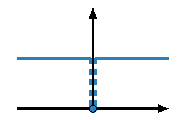
\includegraphics[width=\textwidth]{Figures/l0_regularizer.pdf}
         \caption{$\ell_0$}
     \end{subfigure}%
     \begin{subfigure}[b]{0.25\textwidth}
         \centering
         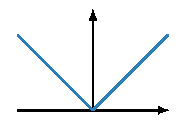
\includegraphics[width=\textwidth]{Figures/l1_regularizer.pdf}
         \caption{$\ell_1$}
     \end{subfigure}%
     \begin{subfigure}[b]{0.25\textwidth}
         \centering
         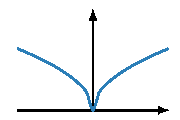
\includegraphics[width=\textwidth]{Figures/lh_regularizer.pdf}
         \caption{$\ell_p,\, p=1/2$}
     \end{subfigure}%
     \begin{subfigure}[b]{0.25\textwidth}
         \centering
         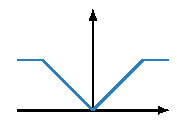
\includegraphics[width=\textwidth]{Figures/scad_regularizer.pdf}
         \caption{SCAD}
     \end{subfigure}
     \caption{Four commonly-used regularizers which promote sparsity}
     \label{fig:three graphs}
\end{figure}

\end{frame}

\begin{frame}{Proximal Gradient Descent for Feature Selection in MLE}
\begin{algorithm}[H]
\TitleOfAlgo{PGD for standard LMEs}
\SetAlgoLined
$\beta^+ \leftarrow\beta_0, \quad \gamma^+\leftarrow\gamma_0, \quad \alpha \leftarrow 1/L$ \tcp*[f]{Initialization}\\
$x^+ = [\beta^+, \gamma^+]$;\\
\While{\text{making progress}}{
	$x^+ \leftarrow \prox_{\alpha^{-1}R + \delta_{\mathcal{C}}}(x^+ - \alpha \nabla_x\LL(x^+))$	\tcp*[f]{PGD iterations}\\	
}
\Return{$x^+ = [\beta^+, \gamma^+]$}
\end{algorithm}
\only<2>{
\vspace{2em}
Basic Assumptions for the PGD Algorithm (Theorem 10.15 from \footcite*{AB17})
\begin{enumerate}
	\item $R$ is a closed proper convex function
	\item $\LL$ is closed and proper, $\dom{\LL}$ convex, $\dom R \subset int(\dom\LL)$, and $\LL$ is $L$-smooth over $int(\dom\LL)$.
	\item The problem has an optimal solution with an optimal value $\LL^*$
\end{enumerate}
}
\only<3>{
	\begin{columns}[T,onlytextwidth]
    \column{0.5\textwidth}
    \vspace{2em}
    Synthetic Benchmark:
    \begin{itemize}
    	\item 100 randomly-generated problems.
    	\item $p = q = 20$.
		\item $\beta = \gamma = \frac{1}{2}[1,2,3,\dots,10, 0\dots,0]$
		\item 9 groups from $3$ to $15$ observations
		\item $X_i \sim \NN(0, I)^p$, $Z_i = X_i$, $\varepsilon_i \sim \NN(0, 0.3^2I)$
		\item Golden search for $\lambda \in [0, 10^5]$
		\item Final model is chosen to maximize BIC
    \end{itemize}
	
    \column{0.5\textwidth}
    	\vspace{1em}
    	\centering  
		\begin{figure}
			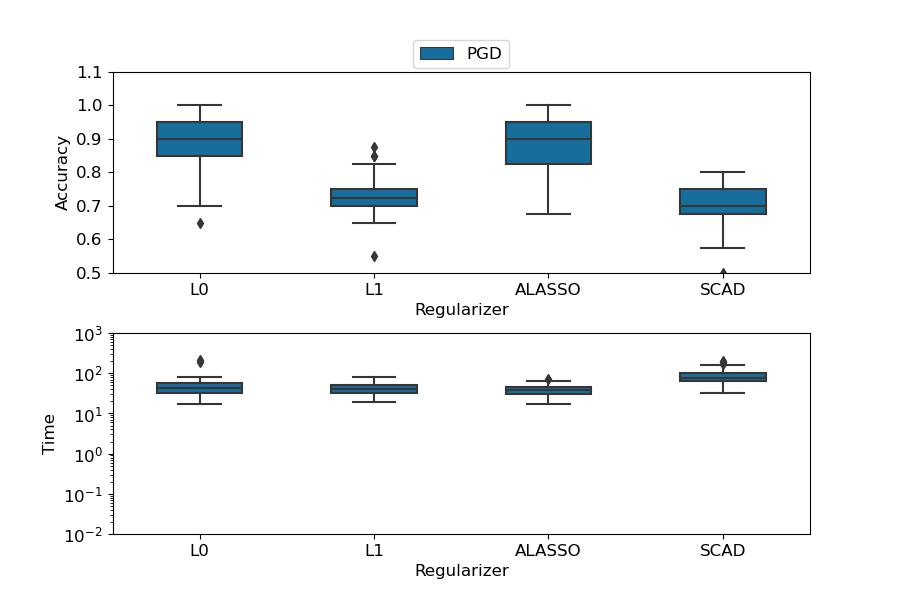
\includegraphics[width=\textwidth]{Figures/benchmark_pgd.jpg}
		\end{figure}
  \end{columns}
}
\end{frame}


\begin{frame}{Sparse Relaxed Regularized Regression ($\mathcal{SR}3$) \footcite{Zheng2018RelaxAndSplit}}
\begin{equation}
	\min_{x} f(x) + R(x)\quad \goto \quad \min_{x, w} f(x) + \frac{\eta}{2} \|x-w\|_2^2 + R(w)
\end{equation}

\begin{figure}
	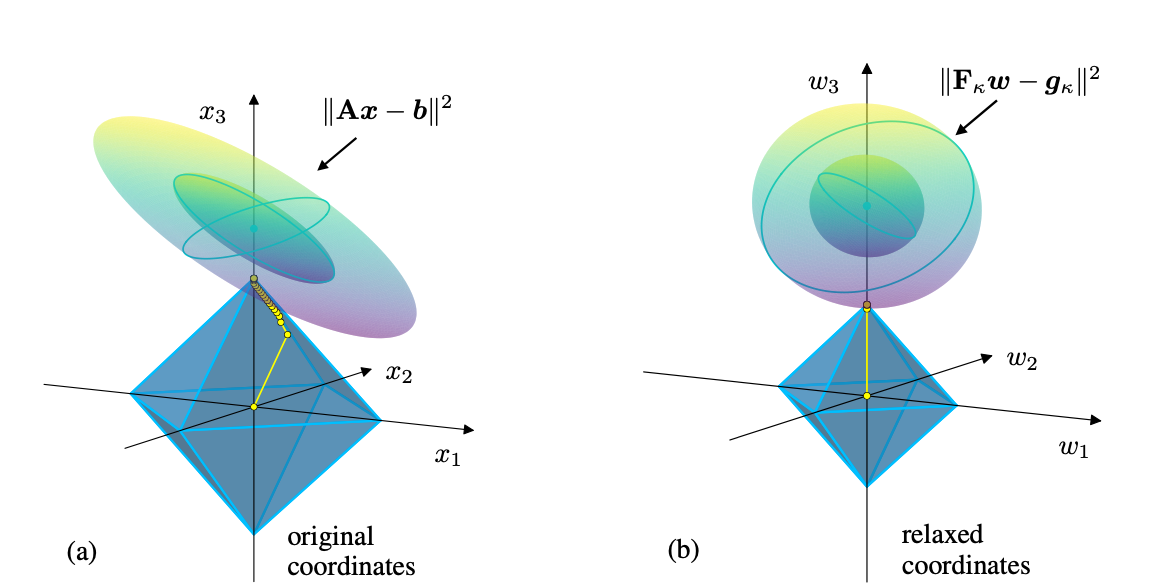
\includegraphics[width=0.7\textwidth]{Figures/intuition_prev_paper.png}
\end{figure}

\textbf{Objectives:}
\begin{itemize}
	\item Extend $\mathcal{SR}3$ relaxation to linear mixed-effects models - $\mathcal{MSR}3$ (see \footcite{sholokhov2022relaxation}).
	\item Develop theoretical foundations for it (see \footcite{aravkin2022jimtheory}).
	\item Implement it as a \texttt{scikit-learn}-compatible Python package -- \texttt{pysr3} (see \footcite{sholokhov2023pysr3}).
\end{itemize}
\vspace{1em}

\end{frame}


\begin{frame}{SR3-Relaxation for Mixed-Effect Models ($\ouralgo$)}
Original problem $\mathcal{FS-LME}$:
\eq{
	\min_{\beta \in \R^p,\, \gamma \in \R^{q}_+} \LL(\beta, \gamma) + R(\beta, \gamma)
}
Relaxed problem $\ouralgo$:
\eq{
	\label{eq:msr3_formulation_explicit}
	\min_{\beta, \tbeta \in \R^p,\, \gamma, \tgamma \in \R^{q}_+} \LL(\beta, \gamma) + \phi_\mu(\gamma) + \kappa_\eta(\beta - \tbeta, \gamma - \tgamma) + R(\tbeta, \tgamma)
}
where the \textit{relaxation} $\kappa_\eta$ decouples the likelihood and the regularizer 
\eq{
	\kappa_\eta(\beta - \tbeta, \gamma - \tgamma) := \frac{\eta}{2}\|\beta - \tbeta\|^2_2 + \frac{\eta}{2}\|\gamma - \tgamma\|_2^2, \quad \eta > \bar\eta
}
and the \textit{perspective mapping} $\phi_\mu$ replaces $\gamma \geq 0$ with a log-barrier 
\eq{
	\phi_\mu(\gamma) := \begin{cases}
		-\mu\sum_{i=1}^q \ln(\gamma_i/\mu), & \mu > 0 \\
		\delta_{\R_+^q}(\gamma), & \mu = 0 \\
		+\infty, & \mu < 0
	\end{cases}
} 
\end{frame}

\begin{frame}{Value Function of $\mathcal{MSR}3$}
$\ouralgo$-relaxation replaces the original likelihood $\LL$ with a \textit{value function} $u_{\eta,\mu}$:
\eq{
	\label{eq:value_function_definition}
	v_{\eta,\mu}(\tbeta,\tgamma) & := \min_{(\beta, \gamma)} \LL_{\eta,\mu}((\beta, \gamma),(\tbeta, \tgamma)) \\  & := \min_{(\beta, \gamma)} \LL(\beta, \gamma) + \phi_\mu(\gamma) + \kappa_\eta(\beta - \tbeta, \gamma - \tgamma)
}
so $\ouralgo$-formulation~(\ref{eq:msr3_formulation_explicit}) becomes
\eq{
	\min_{\tbeta, \tgamma \in \CC} v_{\eta,\mu}(\tbeta, \tgamma) + R(\tbeta, \tgamma)
}

\textbf{NB:} $v_{\eta,\mu}(\tbeta, \tgamma)$ is smooth on $\CC$ and can be evaluated using Interior Point (IP) method

%When $\eta$ is larger than the weak-convexity constant
%\begin{itemize}
%	\item $v_{\eta,\mu}$ is well-defined and continuously differentiable.
%	\item As $\mu \rightarrow 0$ and $\eta \rightarrow \infty$, cluster points of solutions to $\ouralgo$ are first-order stationary points for $\mathcal{FS-LME}$ \\ 
%	\item $v_{\eta, \mu}$ don't need to be evaluated precisely.
%\end{itemize}

% \textbf{Key observation}: in practice, we don't need accurate solutions for~(\ref{eq:value_function_definition}): a few Newton iterations keep the solution close to the central path.
\end{frame}

%\begin{frame}{Value Function Reformulation}
%\begin{figure}
%	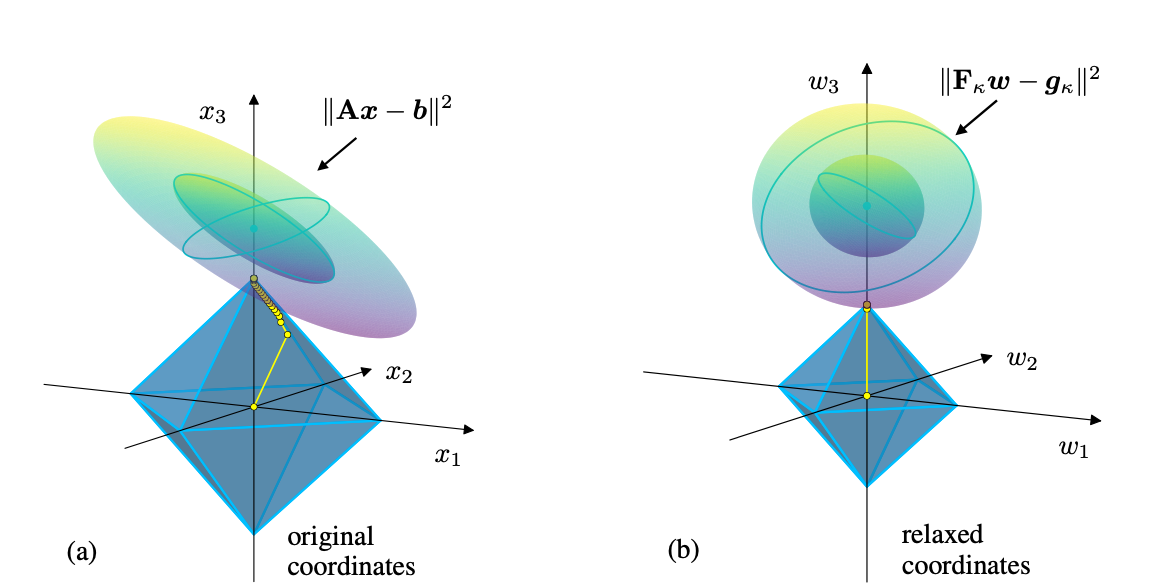
\includegraphics[width=\textwidth]{Figures/intuition_prev_paper}
%	\caption{\label{fig:intuition_prev} Picture from \cite{Zheng2018RelaxAndSplit}: for a linear problem, value function relaxation ``squashes'' level-sets simplifying the optimization landscape.}
%\end{figure}
%\end{frame}

\begin{frame}{Value Function of $\mathcal{MSR}3$}
\[
	\min_{\beta, \gamma \in \CC} \LL(\beta, \gamma) + R(\beta, \gamma) \quad \text{vs} \quad \min_{\tbeta, \tgamma \in \CC} v_{\eta,\mu}(\tbeta, \tgamma) + R(\tbeta, \tgamma)
\]

\begin{figure}
	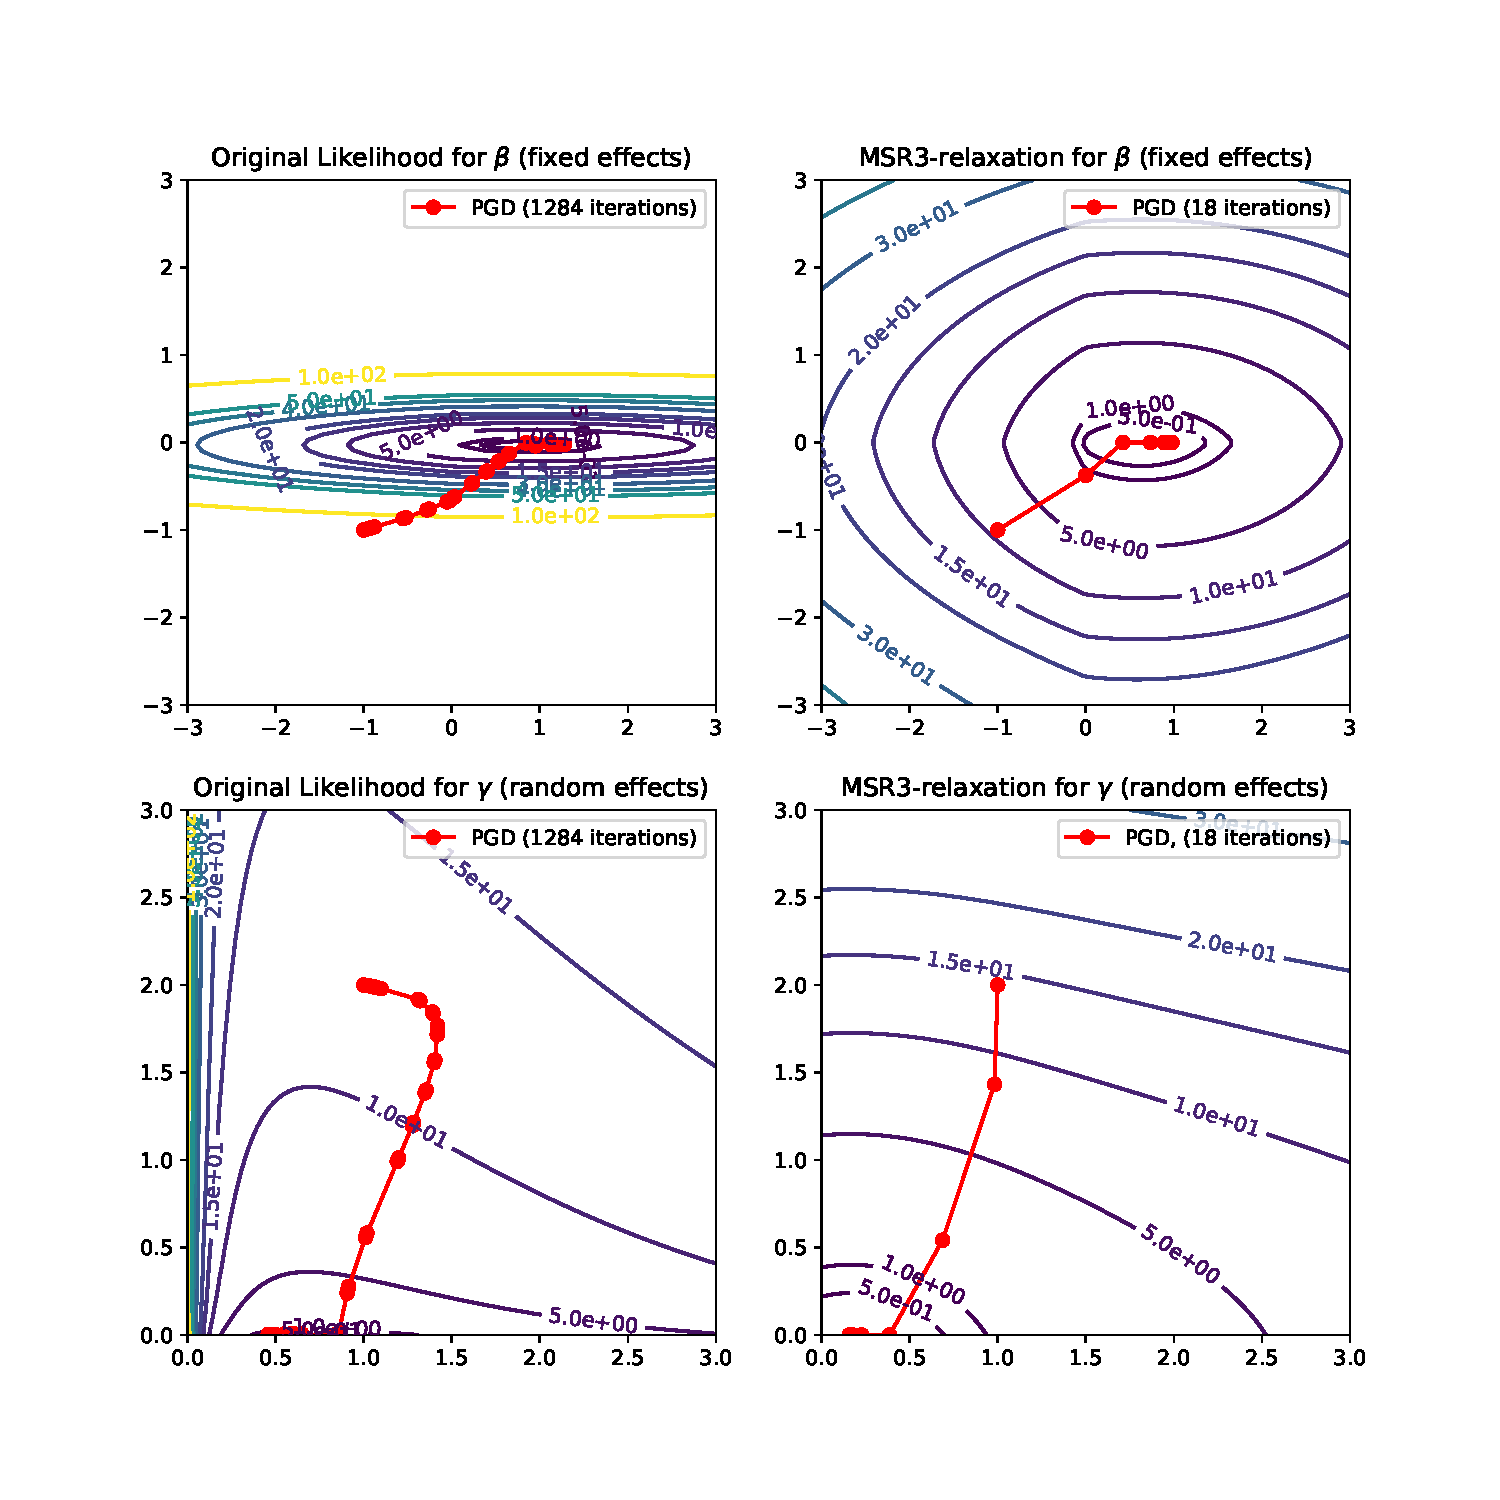
\includegraphics[width=0.7\textwidth]{Figures/intuition_current.pdf}
	\label{fig:intuition_sr3}
\end{figure}
\end{frame}

\begin{frame}{$\mathcal{MSR}3$: Algorithm}

\begin{algorithm}[H]
\TitleOfAlgo{PGD for $\mathcal{MSR}3$}
\SetAlgoLined
$\tbeta^+ \leftarrow \tbeta_0, \quad \tgamma^+ \leftarrow \tgamma_0, \quad \alpha \leftarrow 1/\eta, \quad \eta > \bar{\eta}$ \tcp*[f]{Initialization}\\
$\tw^+ := [\tbeta^+, \tgamma^+], \quad x^+ := [\beta,\gamma]$ \\	
\While{\text{making progress in $\tw$}}{
	\text{$x^+ \leftarrow$ IP solution on $\LL_{\eta,\mu}(x^+, \tw^+)$ s.t. $x^+ \in \CC$} \tcp*[f]{IP Iterations}\\	
	$\nabla_\tw v_{\eta,0}(\tw^+) \leftarrow  \nabla_\tw\LL_{\eta,0}(x^+, \tw^+)$ \tcp*[f]{Evaluate Gradient} \\ 
	$\tw^+ \leftarrow \prox_{\alpha^{-1}R + \delta_{\mathcal{C}}}(\tw^+ - \alpha \nabla_\tw v_{\eta,0}(\tw^+))$	\tcp*[f]{PGD on Value Function}\\
}
\Return{$\tw^+ = [\tbeta^+, \tgamma^+]$}
\end{algorithm}
\only<2>{
\vspace{1em}
Theoretical Results \footcite{aravkin2022jimtheory}:
\begin{enumerate}
	\item The problem has an optimal solution with an optimal value $\Phi^*$ (\textbf{Theorem 5})
	\item $v_{\eta,\mu}$ is well-defined (\textbf{Theorem 5}) and continuously differentiable (\textbf{Theorem 10})
	\item $\nabla v_{\eta,\mu}$ is locally $\widetilde{L}$-continuous when $R$ is 1-coercive (\textbf{Theorem 14})
	\item As $\mu \rightarrow 0$ (\textbf{Theorem 6}) or $\eta \rightarrow \infty$ (\textbf{Theorem 7}), cluster points of solutions to $\ouralgo$ are FOSPs for $\mathcal{FS-LME}$ 
\end{enumerate}
}
\end{frame}

\begin{frame}{$\mathcal{MSR}3$: Results}
    	\centering  
		\begin{figure}
			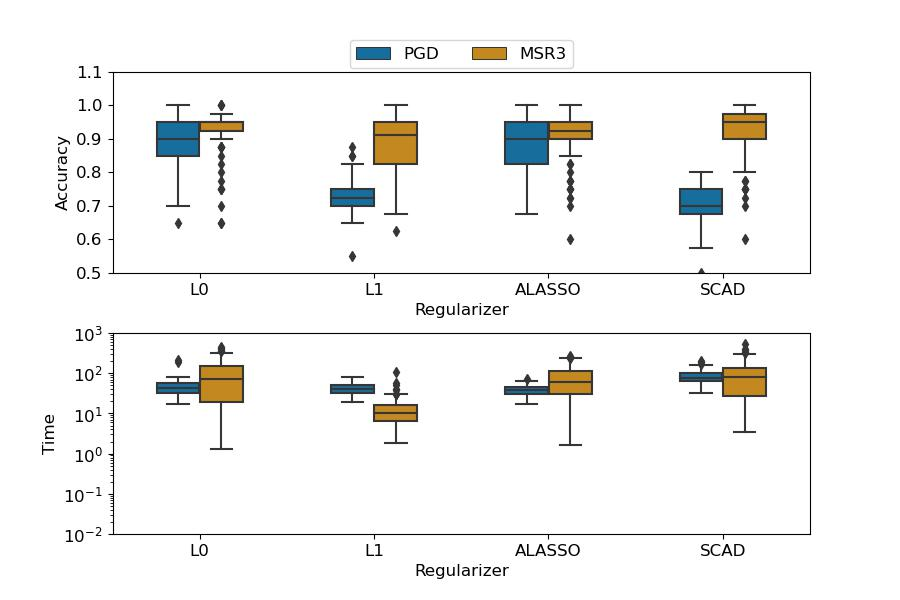
\includegraphics[width=0.7\textwidth]{Figures/benchmark_pgd_msr3.jpg}
		\end{figure}
\end{frame}

\begin{frame}{$\mathcal{MSR}3$: Algorithm}

\begin{algorithm}[H]
\TitleOfAlgo{PGD for $\mathcal{MSR}3$}
\SetAlgoLined
$\tbeta^+ \leftarrow \tbeta_0, \quad \tgamma^+ \leftarrow \tgamma_0, \quad \alpha \leftarrow 1/\eta, \quad \eta > \bar{\eta}$ \tcp*[f]{Initialization}\\
$\tw^+ := [\tbeta^+, \tgamma^+], \quad x^+ := [\beta,\gamma]$ \\	
\While{\text{making progress in $\tw$}}{
	\text{$x^+ \leftarrow$ \textcolor{red}{IP solution on $\LL_{\eta,\mu}(x^+, \tw^+)$ s.t. $x^+ \in \CC$}} \tcp*[f]{IP Iterations}\\	
	$\nabla_\tw v_{\eta,0}(\tw^+) \leftarrow  \nabla_\tw\LL_{\eta,0}(x^+, \tw^+)$ \tcp*[f]{Evaluate Gradient} \\ 
	$\tw^+ \leftarrow \prox_{\alpha^{-1}R + \delta_{\mathcal{C}}}(\tw^+ - \alpha \nabla_\tw v_{\eta,0}(\tw^+))$	\tcp*[f]{PGD on Value Function}\\
}
\Return{$\tw^+ = [\tbeta^+, \tgamma^+]$}
\end{algorithm}
\vspace{2em}
\only<2>{
\textbf{Key Observation:} $\nabla_\tw v(\tw)$ does not need to be evaluated exactly. We only need to come close enough to the central path.
}

\end{frame}


\begin{frame}{$\mathcal{MSR}3$-fast: Algorithm}
\begin{algorithm}[H]
\TitleOfAlgo{$\mathcal{MSR}3$-fast}
\SetAlgoLined
$\tbeta^+ \leftarrow \tbeta_0, \quad \tgamma^+ \leftarrow \tgamma_0, \quad \alpha \leftarrow 1/\eta, \quad \eta > \bar{\eta}$ \tcp*[f]{Initialization}\\
$\tw^+ := [\tbeta^+, \tgamma^+], \quad x^+ := [\beta,\gamma]$ \\	
\While{\text{making progress}}{
	\While{\textcolor{red}{not close enough to the central path}}{
		\text{$x^+ \leftarrow$ IP iteration on $\LL_{\eta,\mu}(x^+, \tw^+)$ s.t. $x^+ \in \CC$} \tcp*[f]{IP Iterations}\\	
	}
	\text{\textcolor{red}{Decrease $\mu$}}\\
	$\nabla_\tw v_{\eta,\mu}(\tw^+) \leftarrow  \nabla_\tw\LL_{\eta,\mu}(x^+, \tw^+)$ \tcp*[f]{Evaluate Gradient} \\ 
	$\tw^+ \leftarrow \prox_{\alpha^{-1}R + \delta_{\mathcal{C}}}(\tw^+ - \alpha \nabla_\tw v_{\eta,\mu}(\tw^+))$	\tcp*[f]{PGD on Value Function}\\
}
\Return{$\tw^+ = [\tbeta^+, \tgamma^+]$}
\end{algorithm}
\end{frame}

\begin{frame}{$\ouralgo$-fast: Results}
\begin{itemize}
	\item The number of fixed effects $p$ and random effects $q$ is 20.
	\item $\beta = \gamma = \frac{1}{2}[1,2,3,\dots,10, 0\dots,0]$
	\item 9 groups with sizes [10, 15, 4, 8, 3, 5, 18, 9, 6]
	\item $X_i \sim \NN(0, I)^p$, $Z_i = X_i$, $\varepsilon_i \sim \NN(0, 0.3^2I)$
	\item Each experiment is repeated 100 times.
	\item Grid-search for $\eta \in [10^{-4}, 10^{2}]$, golden search for $\lambda \in [0, 10^5]$
	\item Final model is chosen to maximize BIC
\end{itemize}
\begin{figure}
	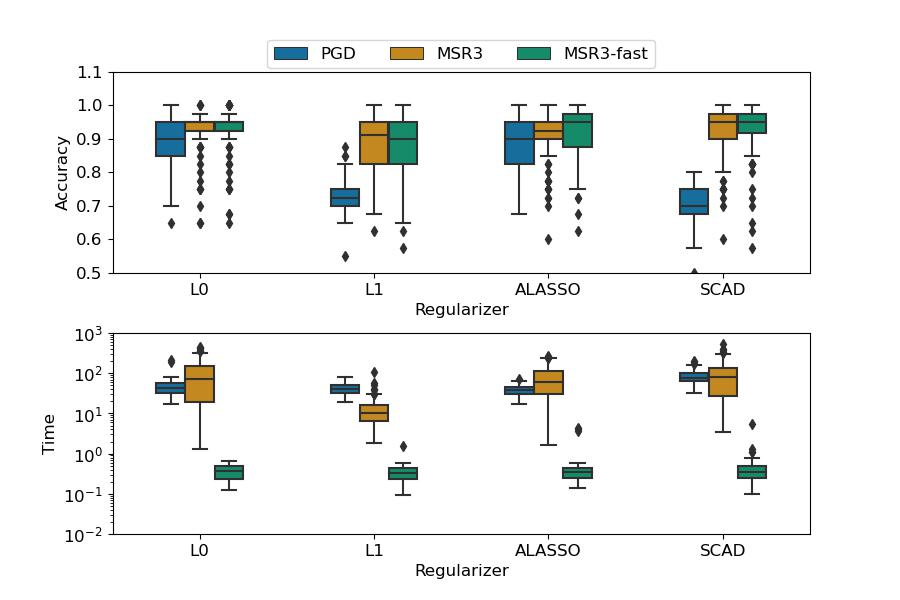
\includegraphics[width=0.7\textwidth]{Figures/benchmark.jpg}
\end{figure}
\begin{itemize}
	\item[\textcolor{green}{+}] $\ouralgo$-relaxation improves feature selection performance of the original likelihood.
	\item[\textcolor{green}{+}] $\ouralgo$-fast optimization accelerates the compute time by $\sim 10^2$.
   	\item[\textcolor{red}{--}] Initialization of $\eta$ is problem-specific
\end{itemize}
\end{frame}

\begin{frame}{Comparison to Other Libraries}
\begin{table}
	\begin{tabular}{lrrrr}
\toprule
Algorithm &        MSR3-Fast ($\ell_1$)&         \texttt{glmmLasso}\footnote{\href{https://rdrr.io/cran/glmmLasso/man/glmmLasso.html}{https://rdrr.io/cran/glmmLasso/man/glmmLasso.html}} \cite{groll2014variable}  &            \texttt{lmmLasso}\footnote{\href{https://rdrr.io/cran/lmmlasso/}{https://rdrr.io/cran/lmmlasso/}}\cite{schelldorfer2011estimation} & PGD ($\ell_1$) \\
\midrule
Accuracy, \% &     {\bf 88} &        48 &          66 & 73  \\
FE Accuracy, \% &      {\bf 86} &        52  &          47 & 56\\
RE Accuracy, \% &     {\bf 91} &        45  &         84 & {\bf 91} \\
Time, sec        & {\bf 0.19} &  1.37  &  11.51 & 38.39 \\
Iterations, num  &      34 &        50 &             - & 7693 \\
\bottomrule
\end{tabular}
\end{table}
\end{frame}

\begin{frame}{Choice of $\eta$}
	\begin{figure}
		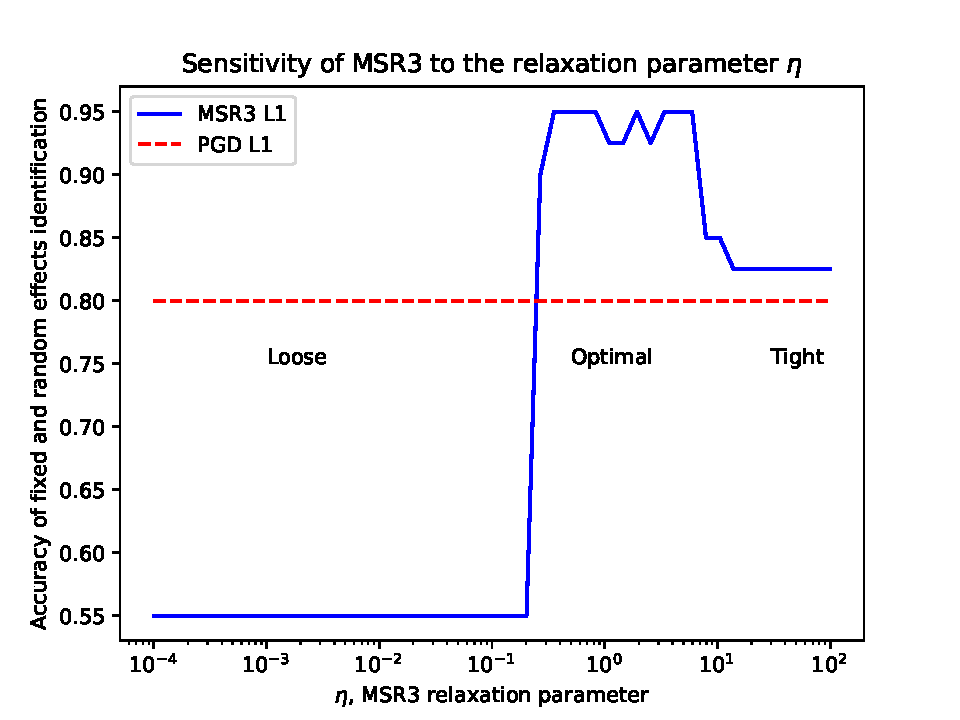
\includegraphics[width=\textwidth]{Figures/eta_L1.pdf}
	\end{figure}
\end{frame}

\begin{frame}{$\ell_0$-based Covariate Selection for Bullying Study from GBD}
	\begin{figure}
		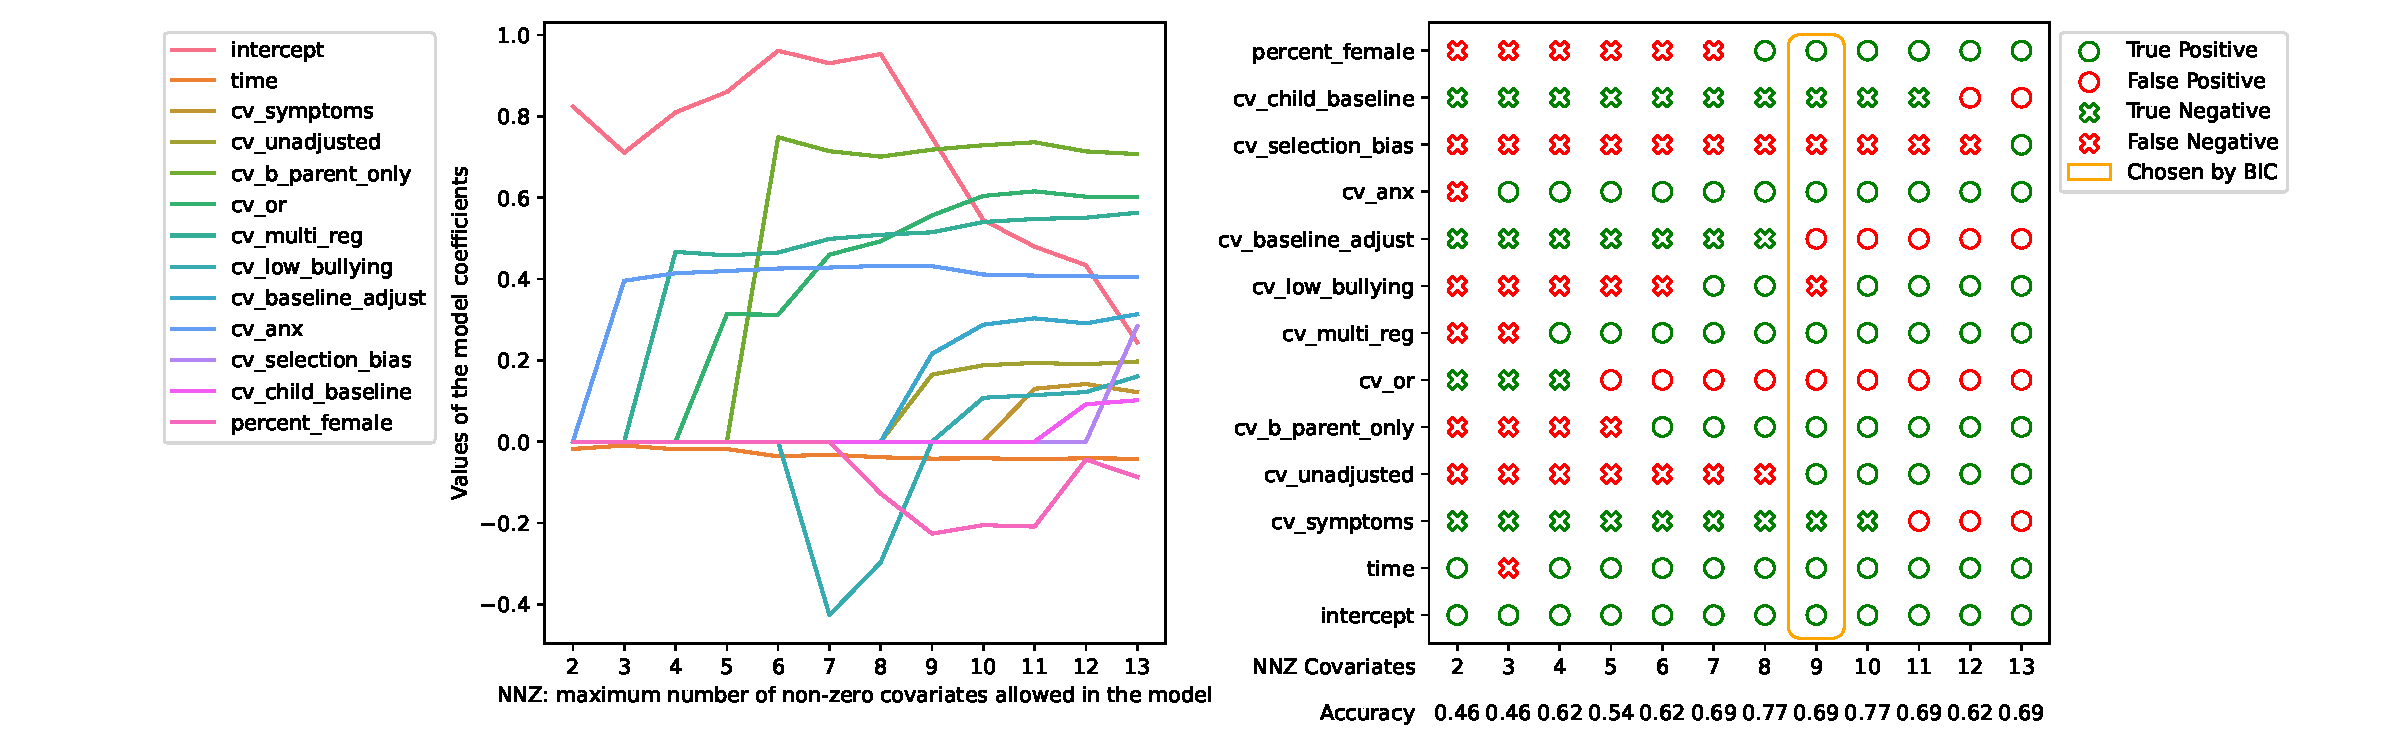
\includegraphics[width=\textwidth]{Figures/bullying_data_assessment_selection.pdf}
		\caption{Fixed and random covariate selection for Bullying dataset\footnote{Institute for Health Metrics and Evaluation (IHME). Bullying Victimization Relative Risk Bundle GBD 2020. Seattle, United States of America (USA), 2021.}. The model selected 9 covariates, 7 of which were historically significant, and did not select 4 covariates, 1 of which was historically significant.}
	\end{figure}
\end{frame}

\begin{frame}{Software}
	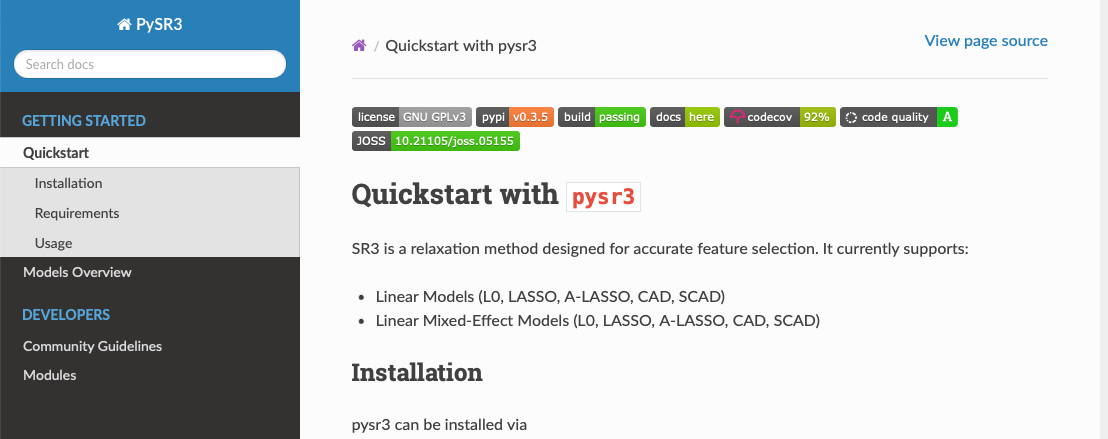
\includegraphics[width=\textwidth]{Figures/pysr3_screenshot.png}
	The code is available on GitHub: \href{github.com/aksholokhov/pysr3}{https://github.com/aksholokhov/pysr3}\footfullcite{sholokhov2023pysr3}
	\begin{itemize}
		\item All estimators are fully compatible to \texttt{scikit-learn} library.
		\item Implements SR3 for linear, generalized-linear, and linear mixed-effect models.
		\item Has tutorials, tests, and documentation.
	\end{itemize}
\end{frame}

\section{Physics-Informed Neural ODE (PINODE): Embedding Physics into Models using Collocation Points}

\subsection{Intro to Physics-Informed Reduced-Order Models (ROMs)}

\begin{frame}{Data-Driven Modeling of Physical Systems}

%1) People used to model physical systems with first-principle knowledge
%2) Data-Driven modelling of dynamical systems became a big thing  
%3) However, it requires a lot of data 
%4) Incorporating prior knowledge is a big recent trend, so history does a spiral

\uncover<2->{
\begin{columns}[T,onlytextwidth]
\column{0.6\textwidth}
\textcolor{orange}{First-Principle Models:}
\begin{itemize}
	\item Require extensive knowledge of the phenomenon
	\item Require a lot of compute for simulating large-scale phenomena
\end{itemize}
\column{0.4\textwidth}
\centering
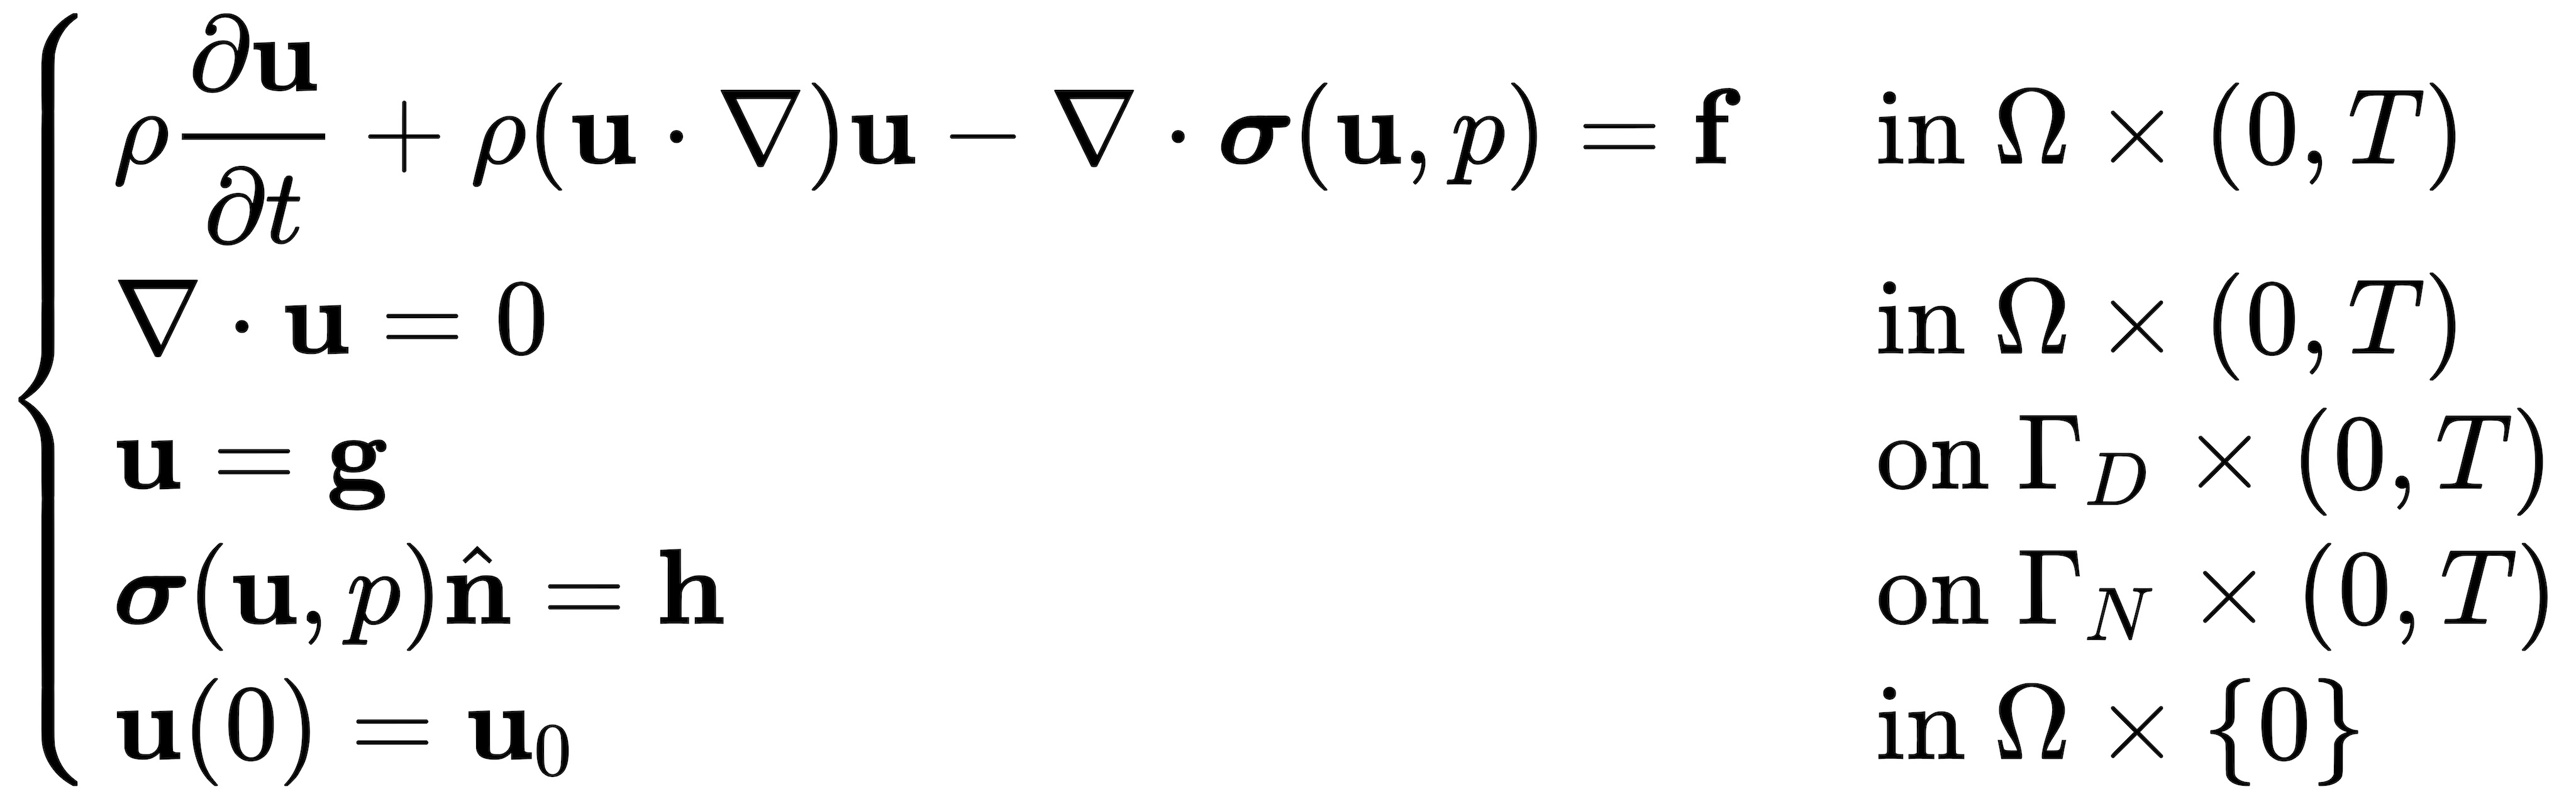
\includegraphics[width=\textwidth]{Figures/NN.jpg}
\end{columns}
}
\vspace{2em}
\uncover<3->{
\begin{columns}[T,onlytextwidth]
\column{0.6\textwidth}
\textcolor{green}{Data-Driven Models:}
\begin{itemize}
	\item Require a lot of data
	\item Often struggle to extrapolate
\end{itemize}
\column{0.4\textwidth}
\centering
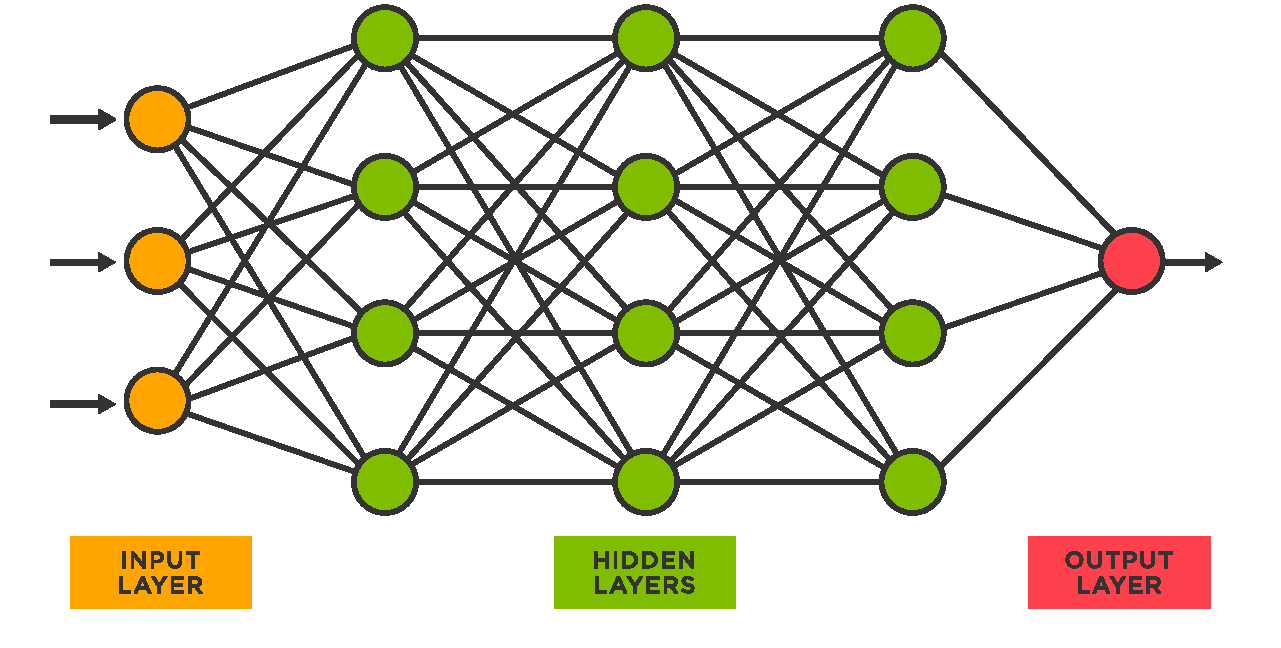
\includegraphics[width=0.8\textwidth]{Figures/nn_schematics.pdf}
\end{columns}
}
\vspace{2em}
\uncover<4->{
\begin{columns}[T,onlytextwidth]
\column{0.6\textwidth}
\textcolor{blue}{Hybrid Models: }
\begin{itemize}
	\item Incorporate elements of both approaches
	\item Supplement data with knowledge or priors
\end{itemize}
\column{0.4\textwidth}
\centering
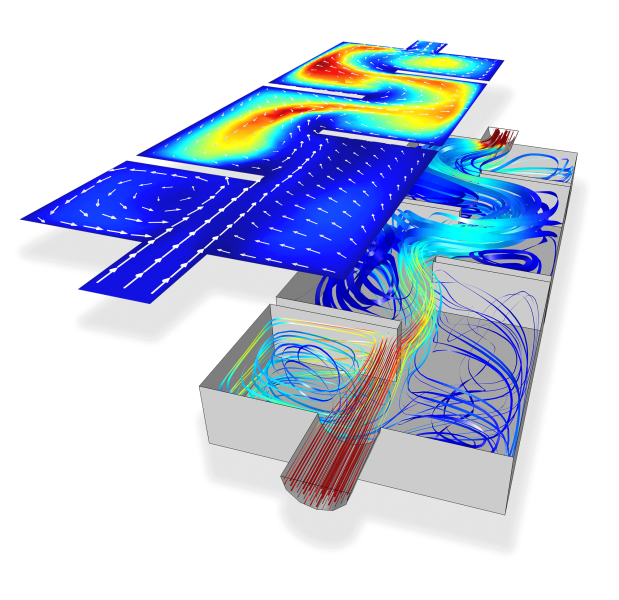
\includegraphics[width=0.7\textwidth]{Figures/NS_pic.png}
\end{columns}
}
\end{frame}

\begin{frame}{Incorporating Knowledge of Physics into Neural Networks}
\begin{enumerate}
	\item<2-> \textbf{Symmetry Based:} incorporate symmetries and conservation laws as hard constraints into a network: E3NNs\footcite{geiger2022e3nn}, LieConv\footcite{Finzi2020}, RiCNN \footcite{chidester2018rotation}
	\item<3-> \textbf{Model Discovery Based:} use a library of terms to discover simple equations: SINDy\footcite{champion2019data}, Genetic Programming\footcite{schmidt2009distilling}
	\item<4-> \textbf{Equations Based:} incorporate first-principle models to aid training of networks: PINNs\footcite{raissi2017physics}, UDEs\footcite{rackauckas2020udes}
\end{enumerate}

\begin{columns}[T,onlytextwidth]
\column{0.3\textwidth}
	\uncover<2->{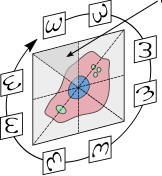
\includegraphics[width=0.7\textwidth]{Figures/ricnn.png}}
\column{0.7\textwidth}
	\uncover<3->{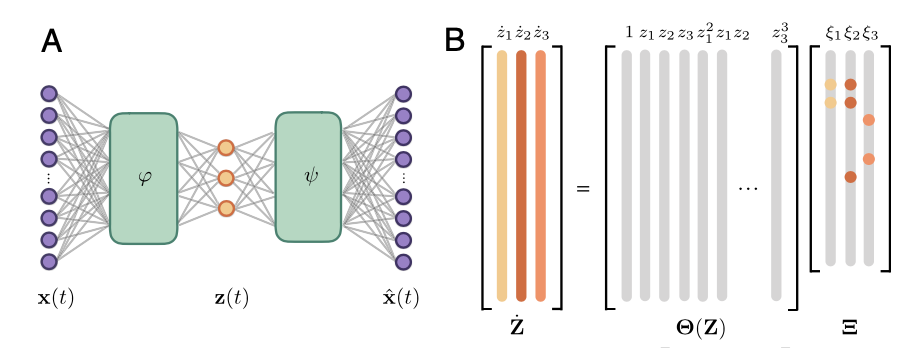
\includegraphics[width=\textwidth]{Figures/sindy.png}}
\end{columns}

\end{frame}


\begin{frame}{Reduced-Order Models (ROMs)}
\only<1>{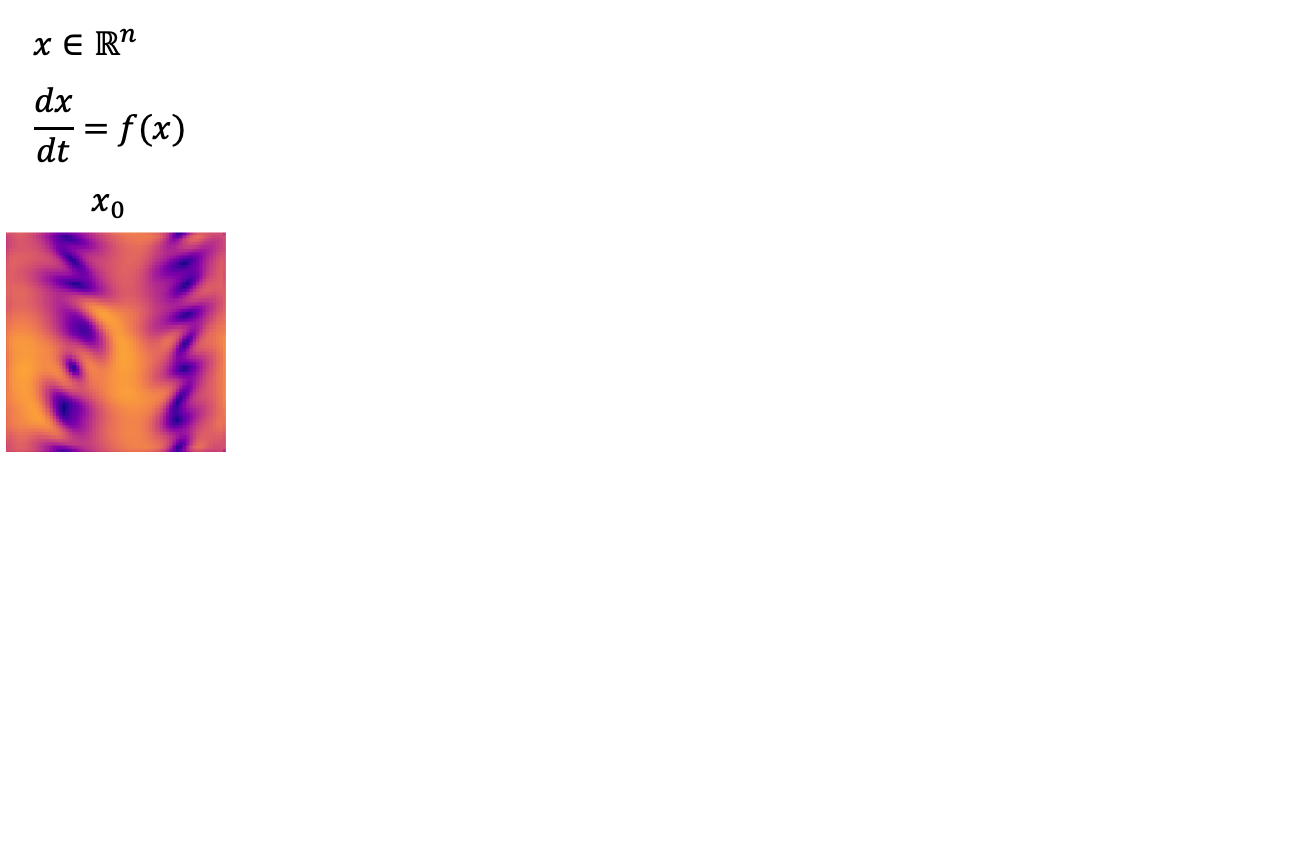
\includegraphics[width=\textwidth]{Figures/roms_1}}
\only<2>{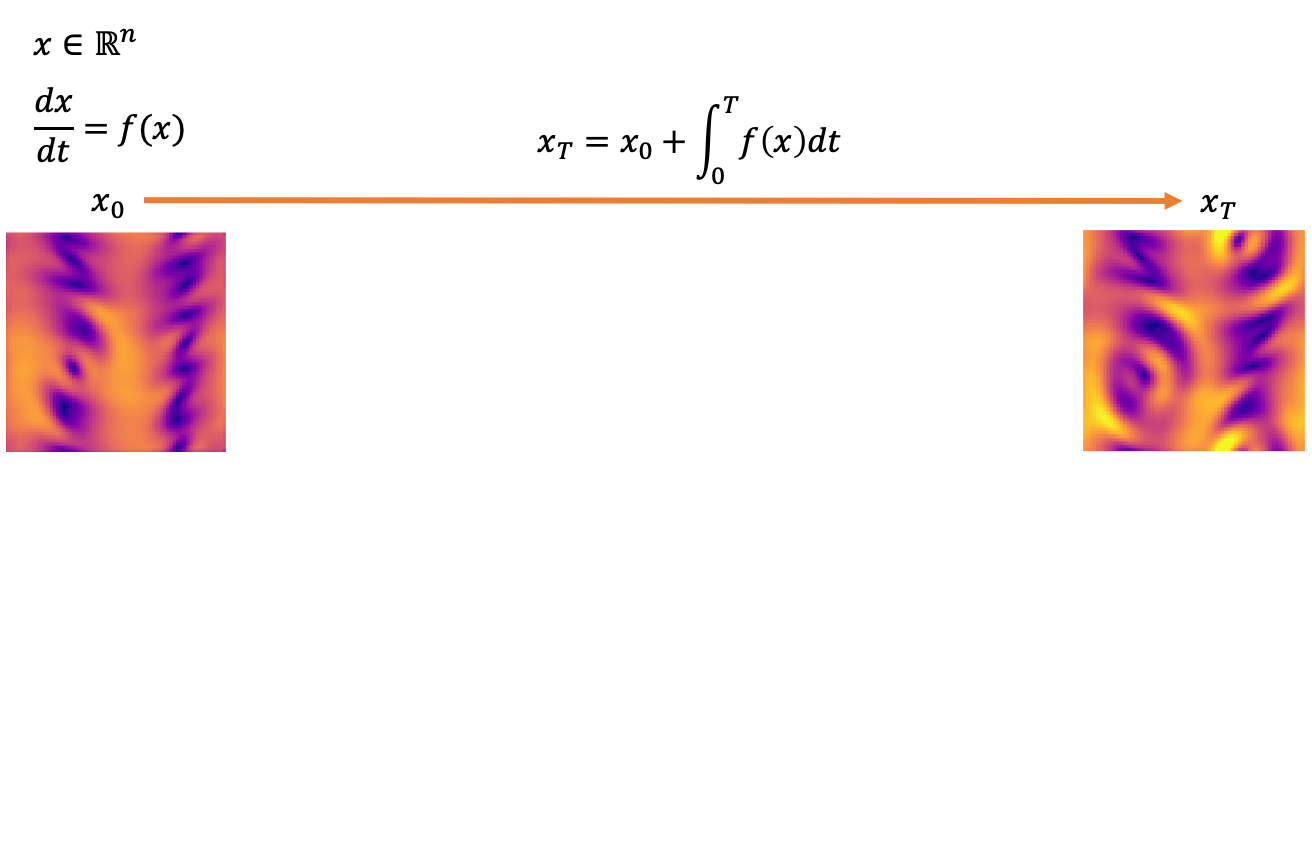
\includegraphics[width=\textwidth]{Figures/roms_2}}
\only<3>{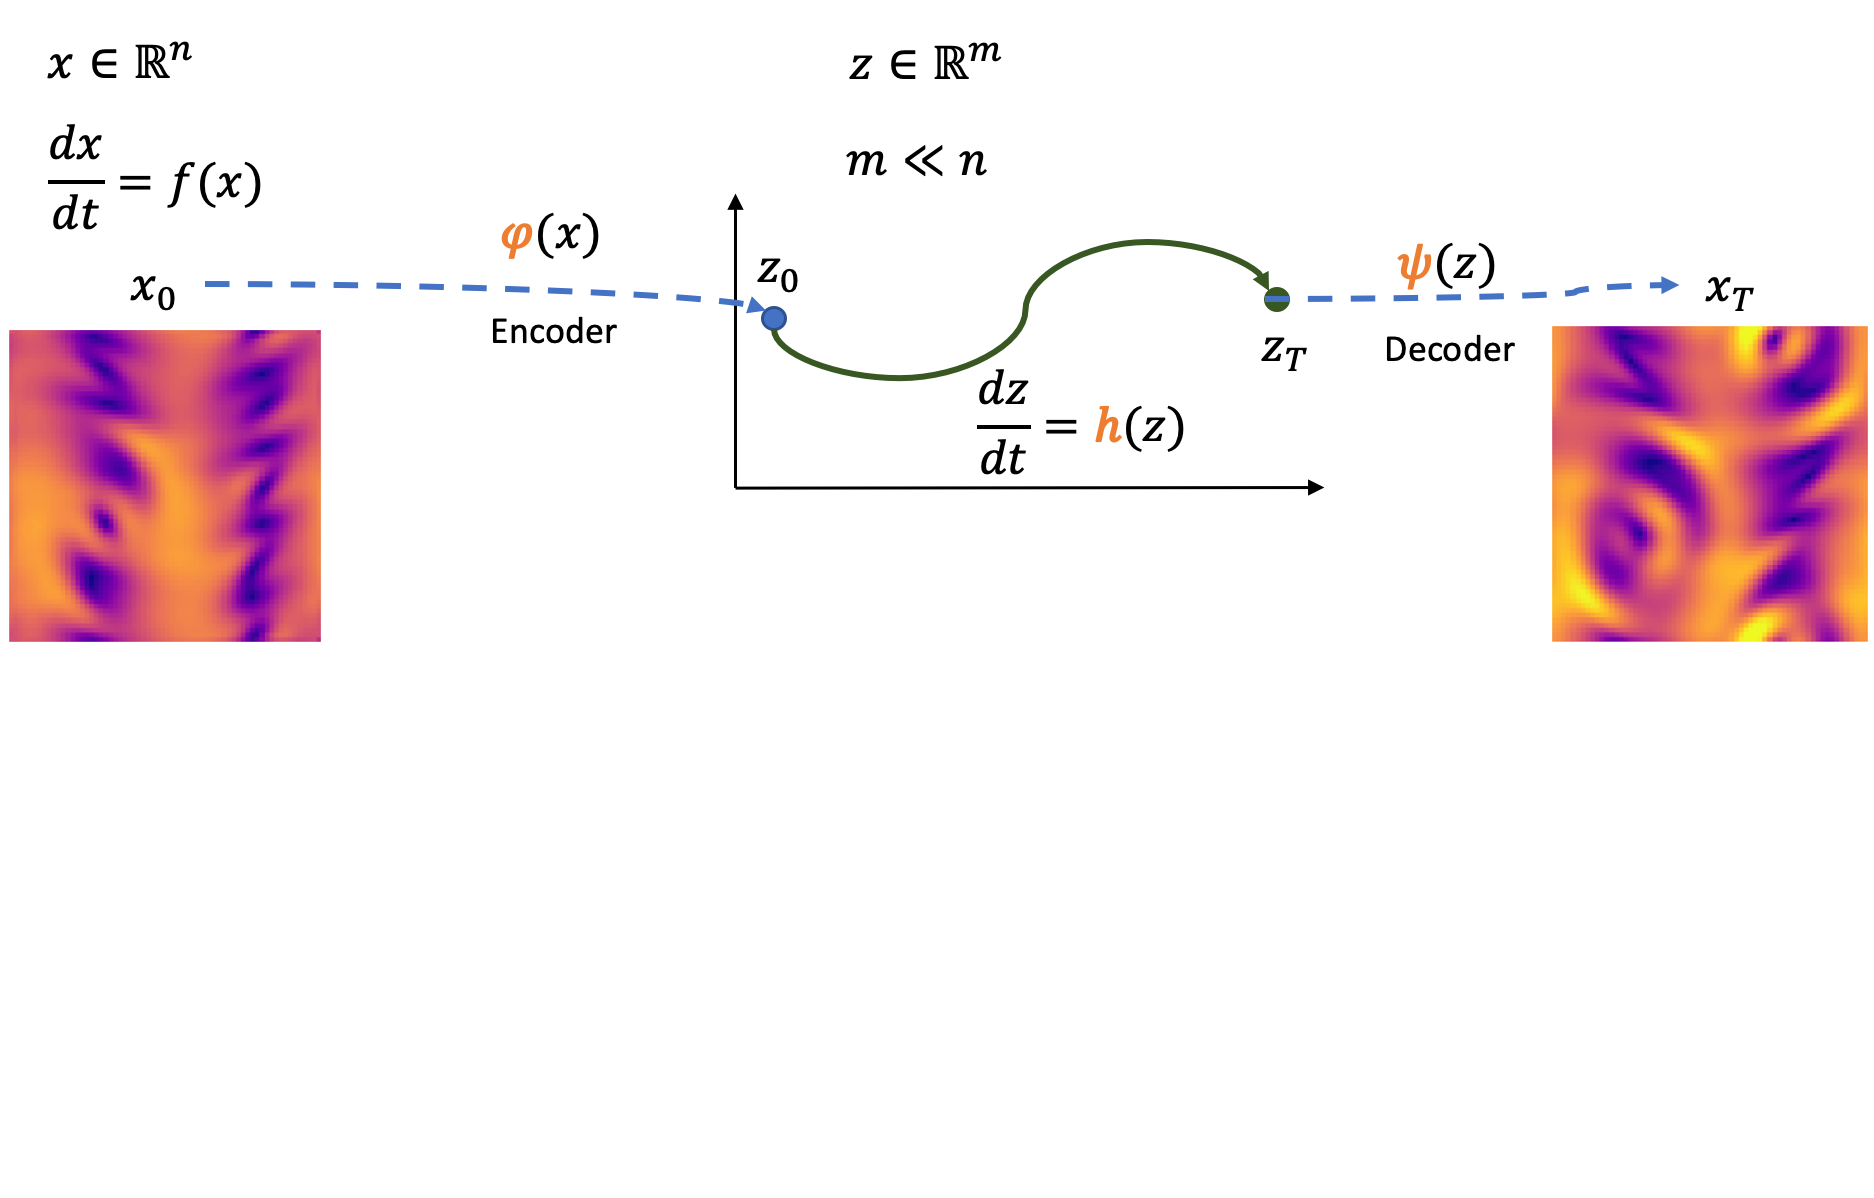
\includegraphics[width=\textwidth]{Figures/roms_3}}
\only<4>{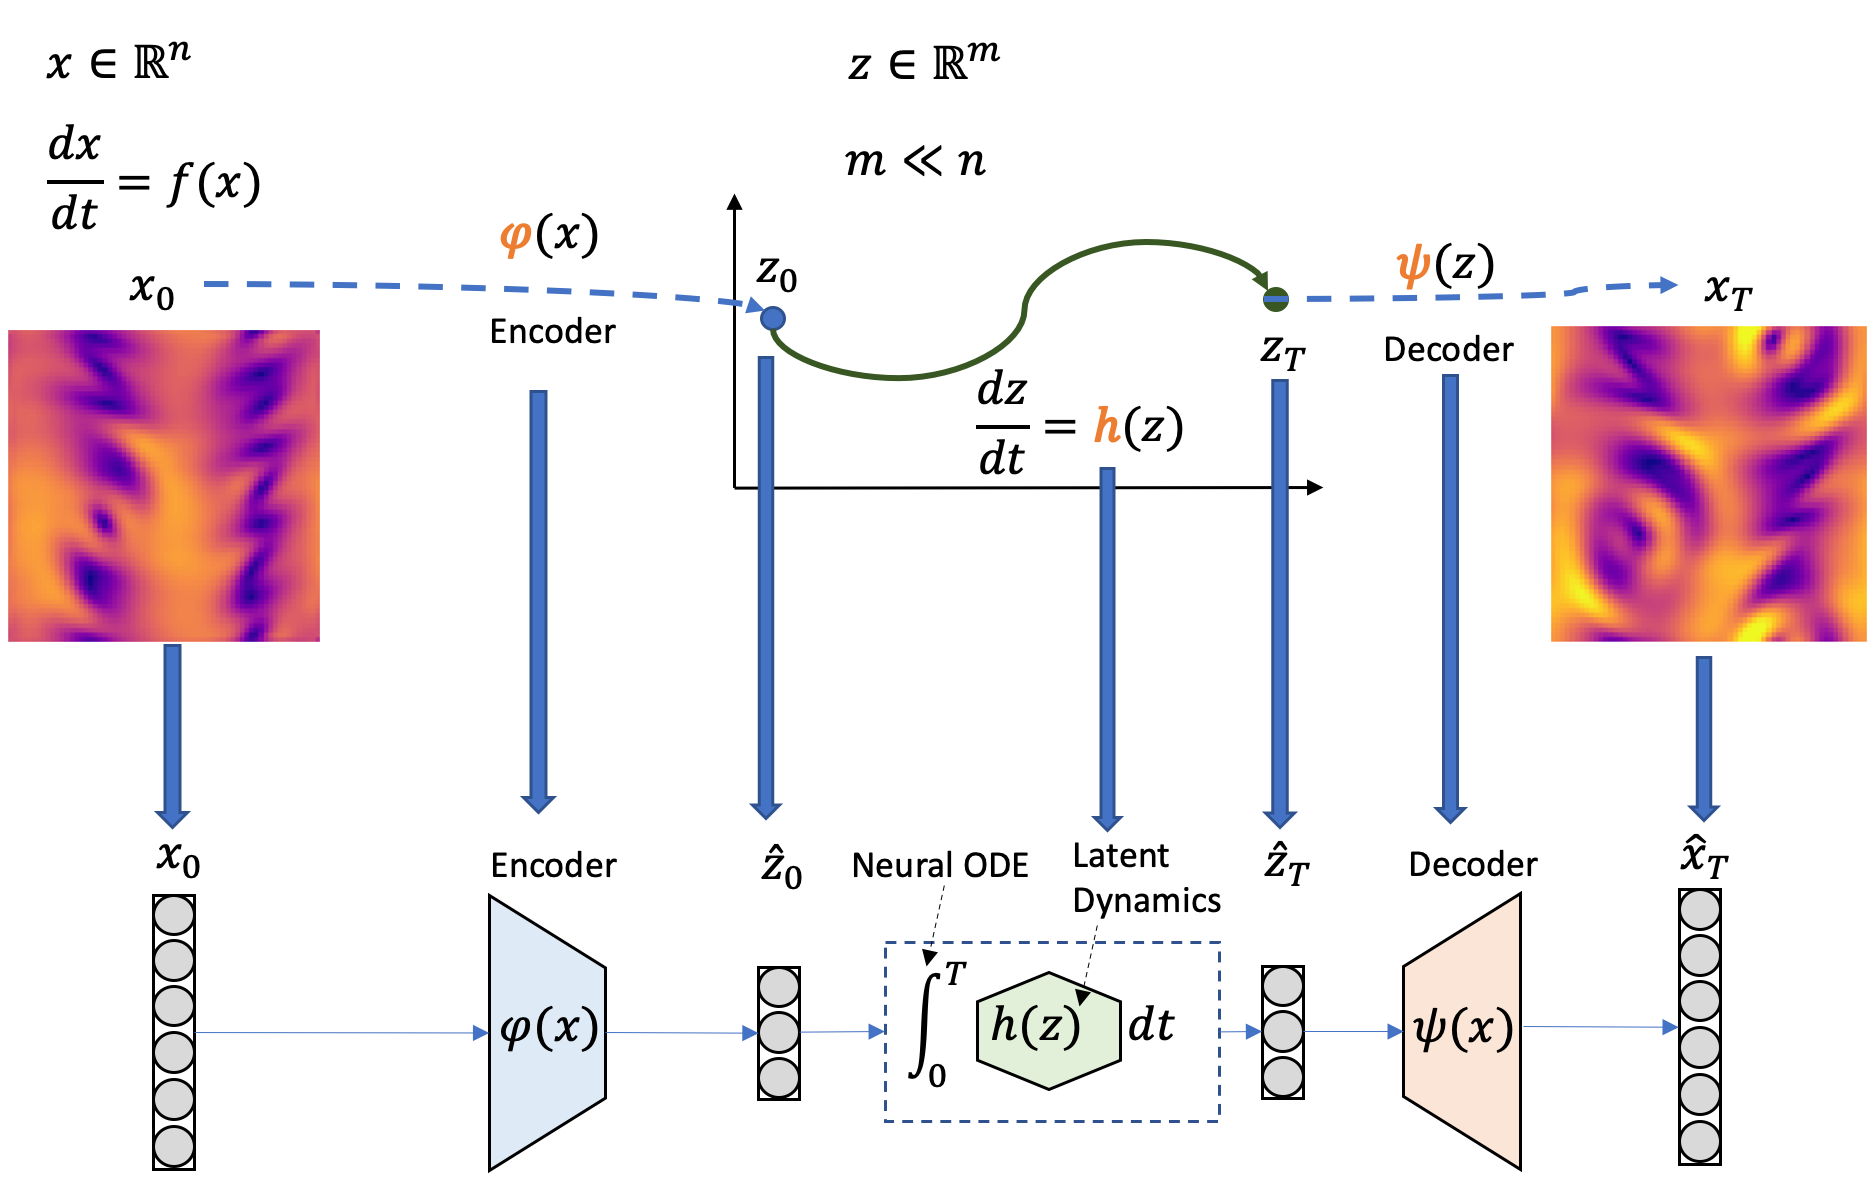
\includegraphics[width=\textwidth]{Figures/roms_4}}
\end{frame}

\begin{frame}{Physics-Informed Loss}
%1) We introduce physics to this system by adding a term which regularizes latent gradient field. 
%2) In particular, it forces it to be equal to what a true physics should be under such projection.
%3) We can not evaluate physics everywhere but we can at particular carefully-selected points. We call these points collocation points.
%4) We feed a lot of collocation points and ask a network to do interpolation 
Using chain rule:
\only<1>{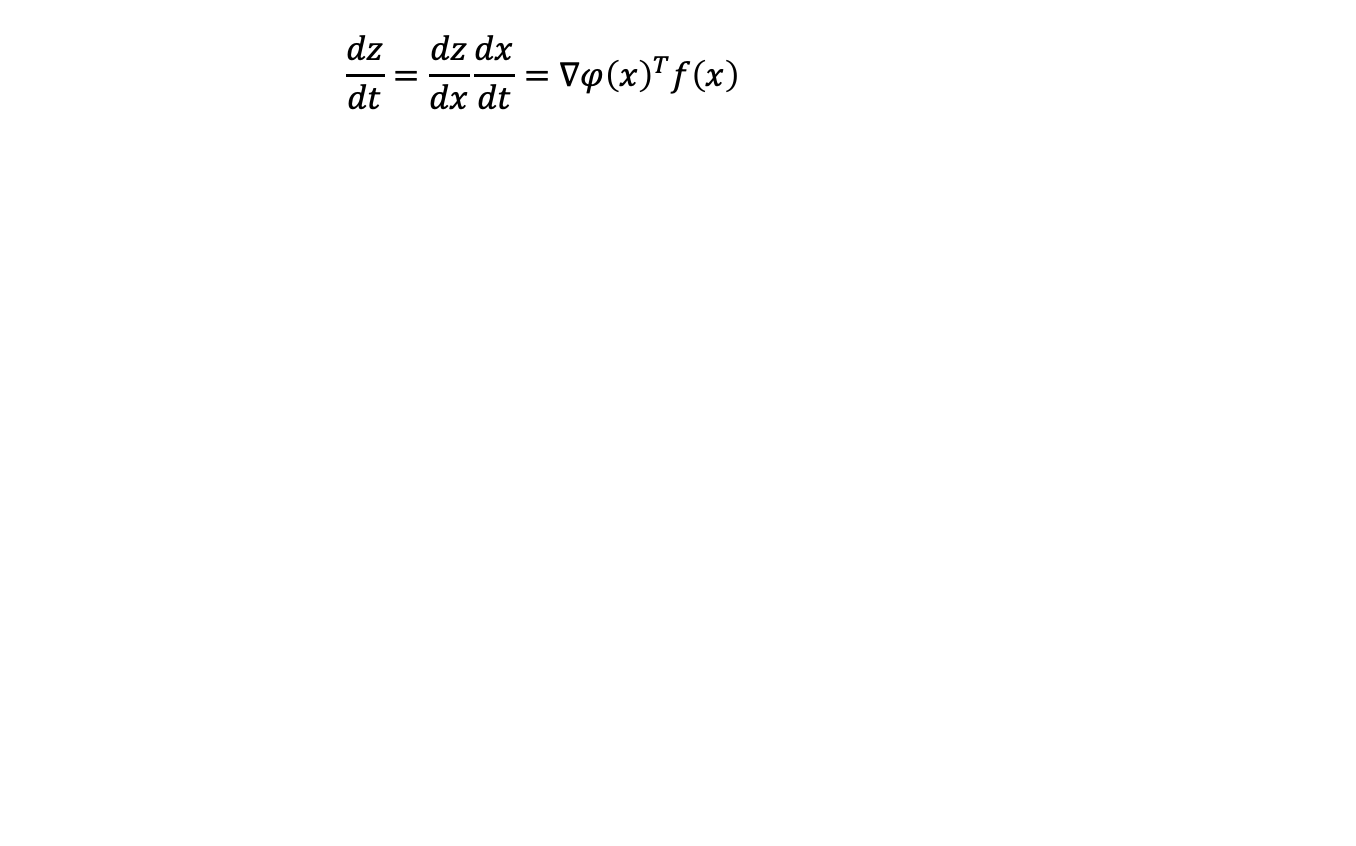
\includegraphics[width=\textwidth]{Figures/collocations_1.png}}
\only<2>{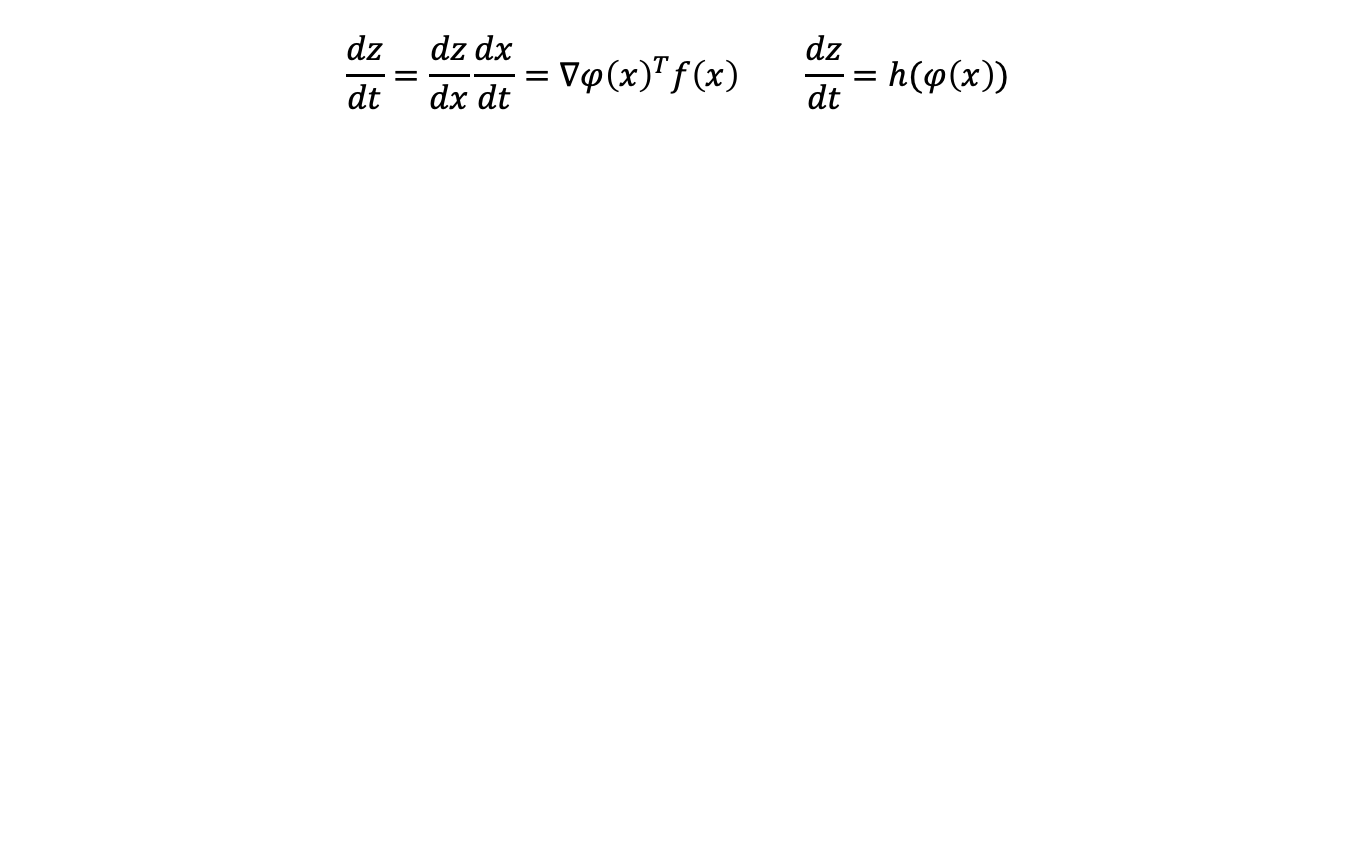
\includegraphics[width=\textwidth]{Figures/collocations_2.png}}
\only<3>{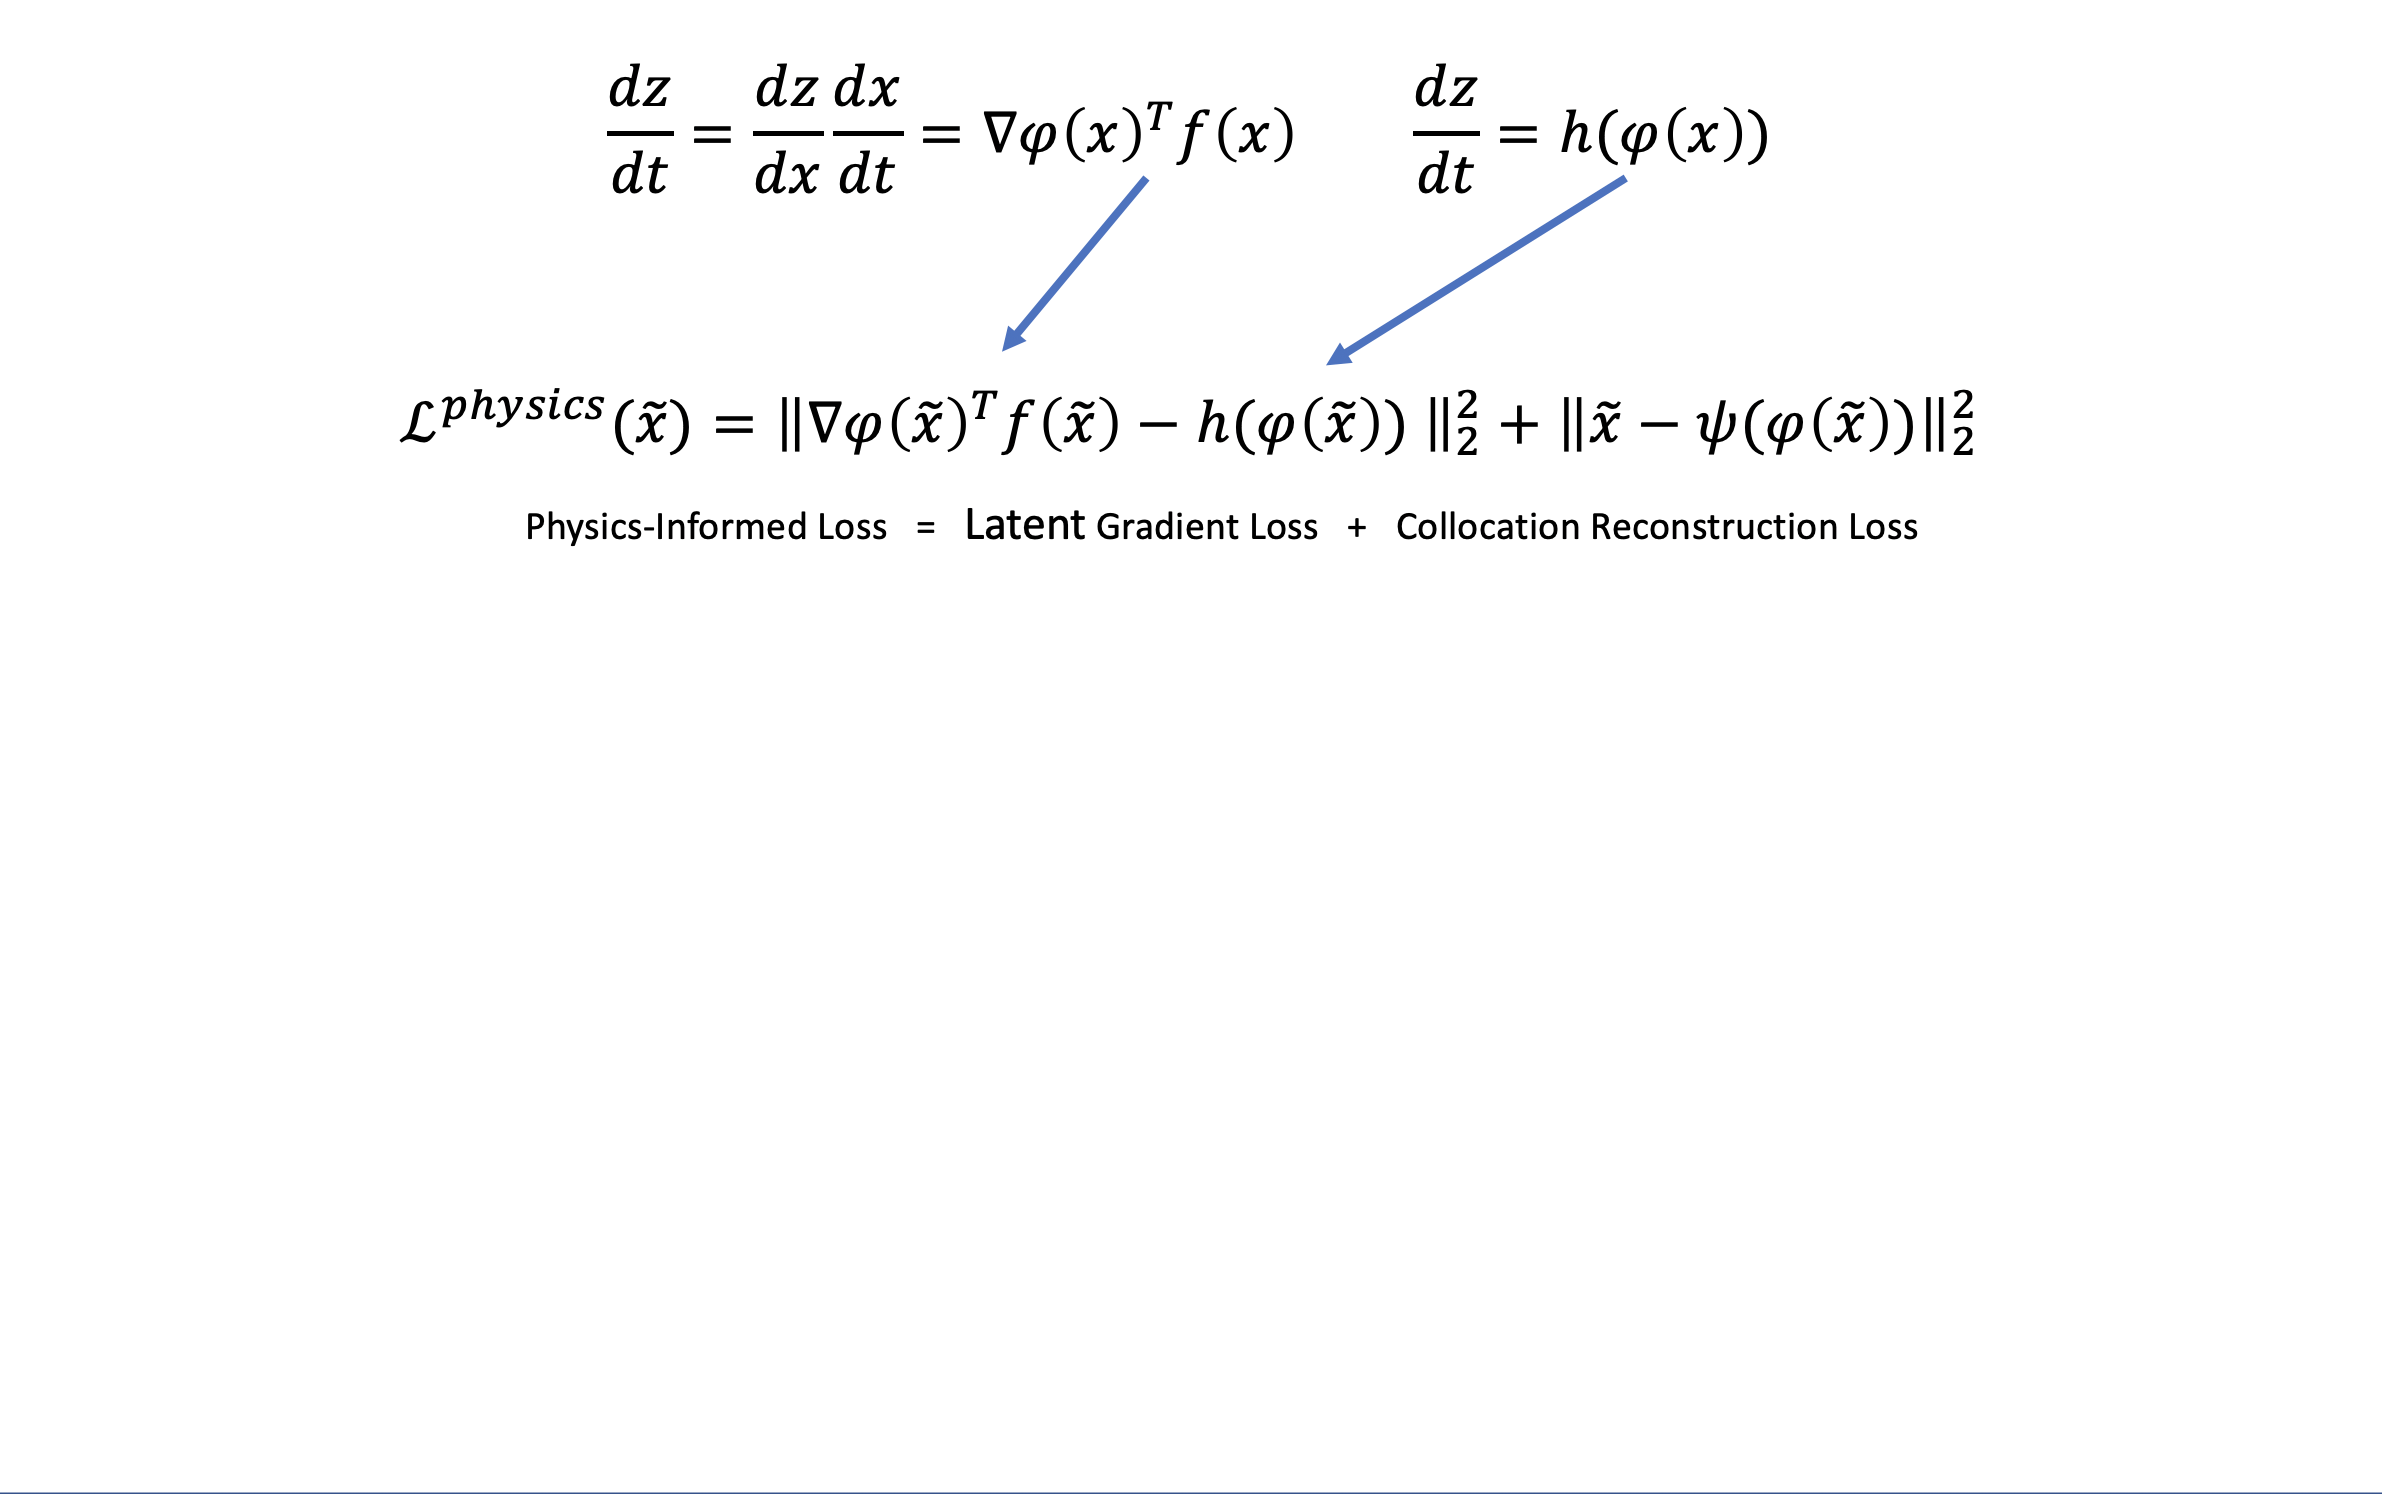
\includegraphics[width=\textwidth]{Figures/collocations_3.png}}
\only<4>{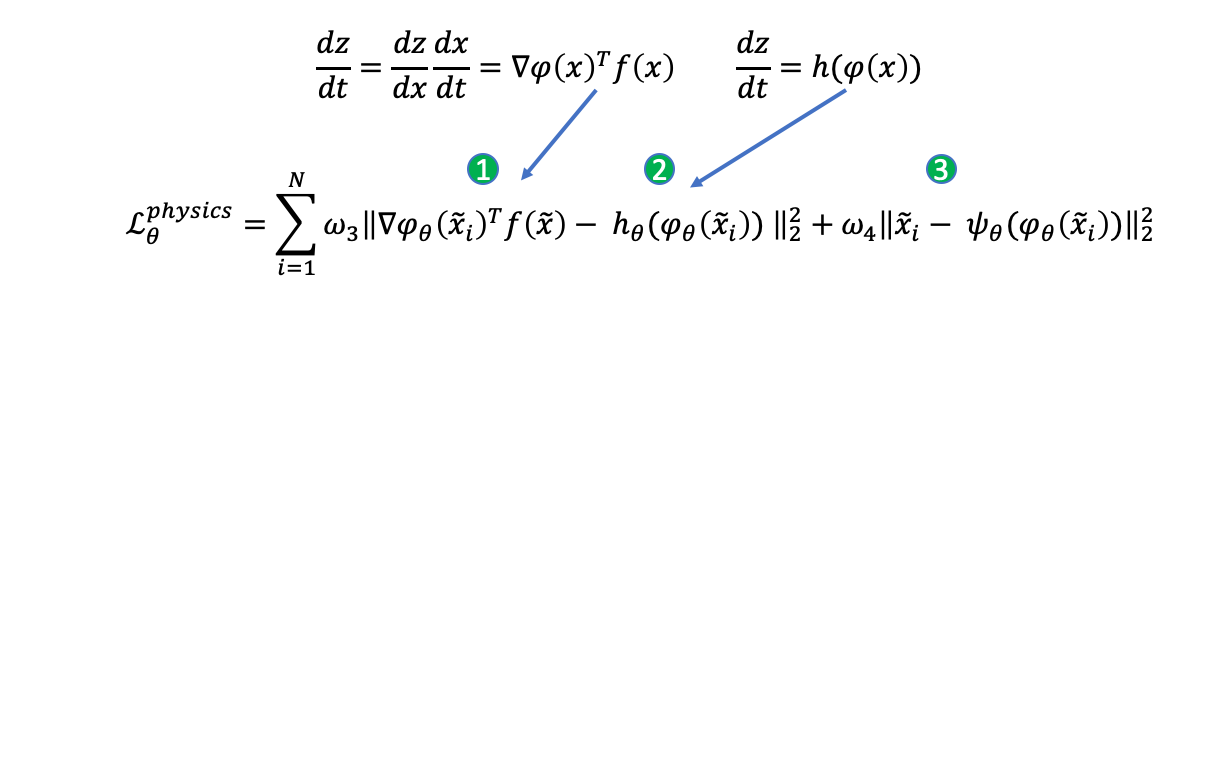
\includegraphics[width=\textwidth]{Figures/collocations_4.png}}
\only<5>{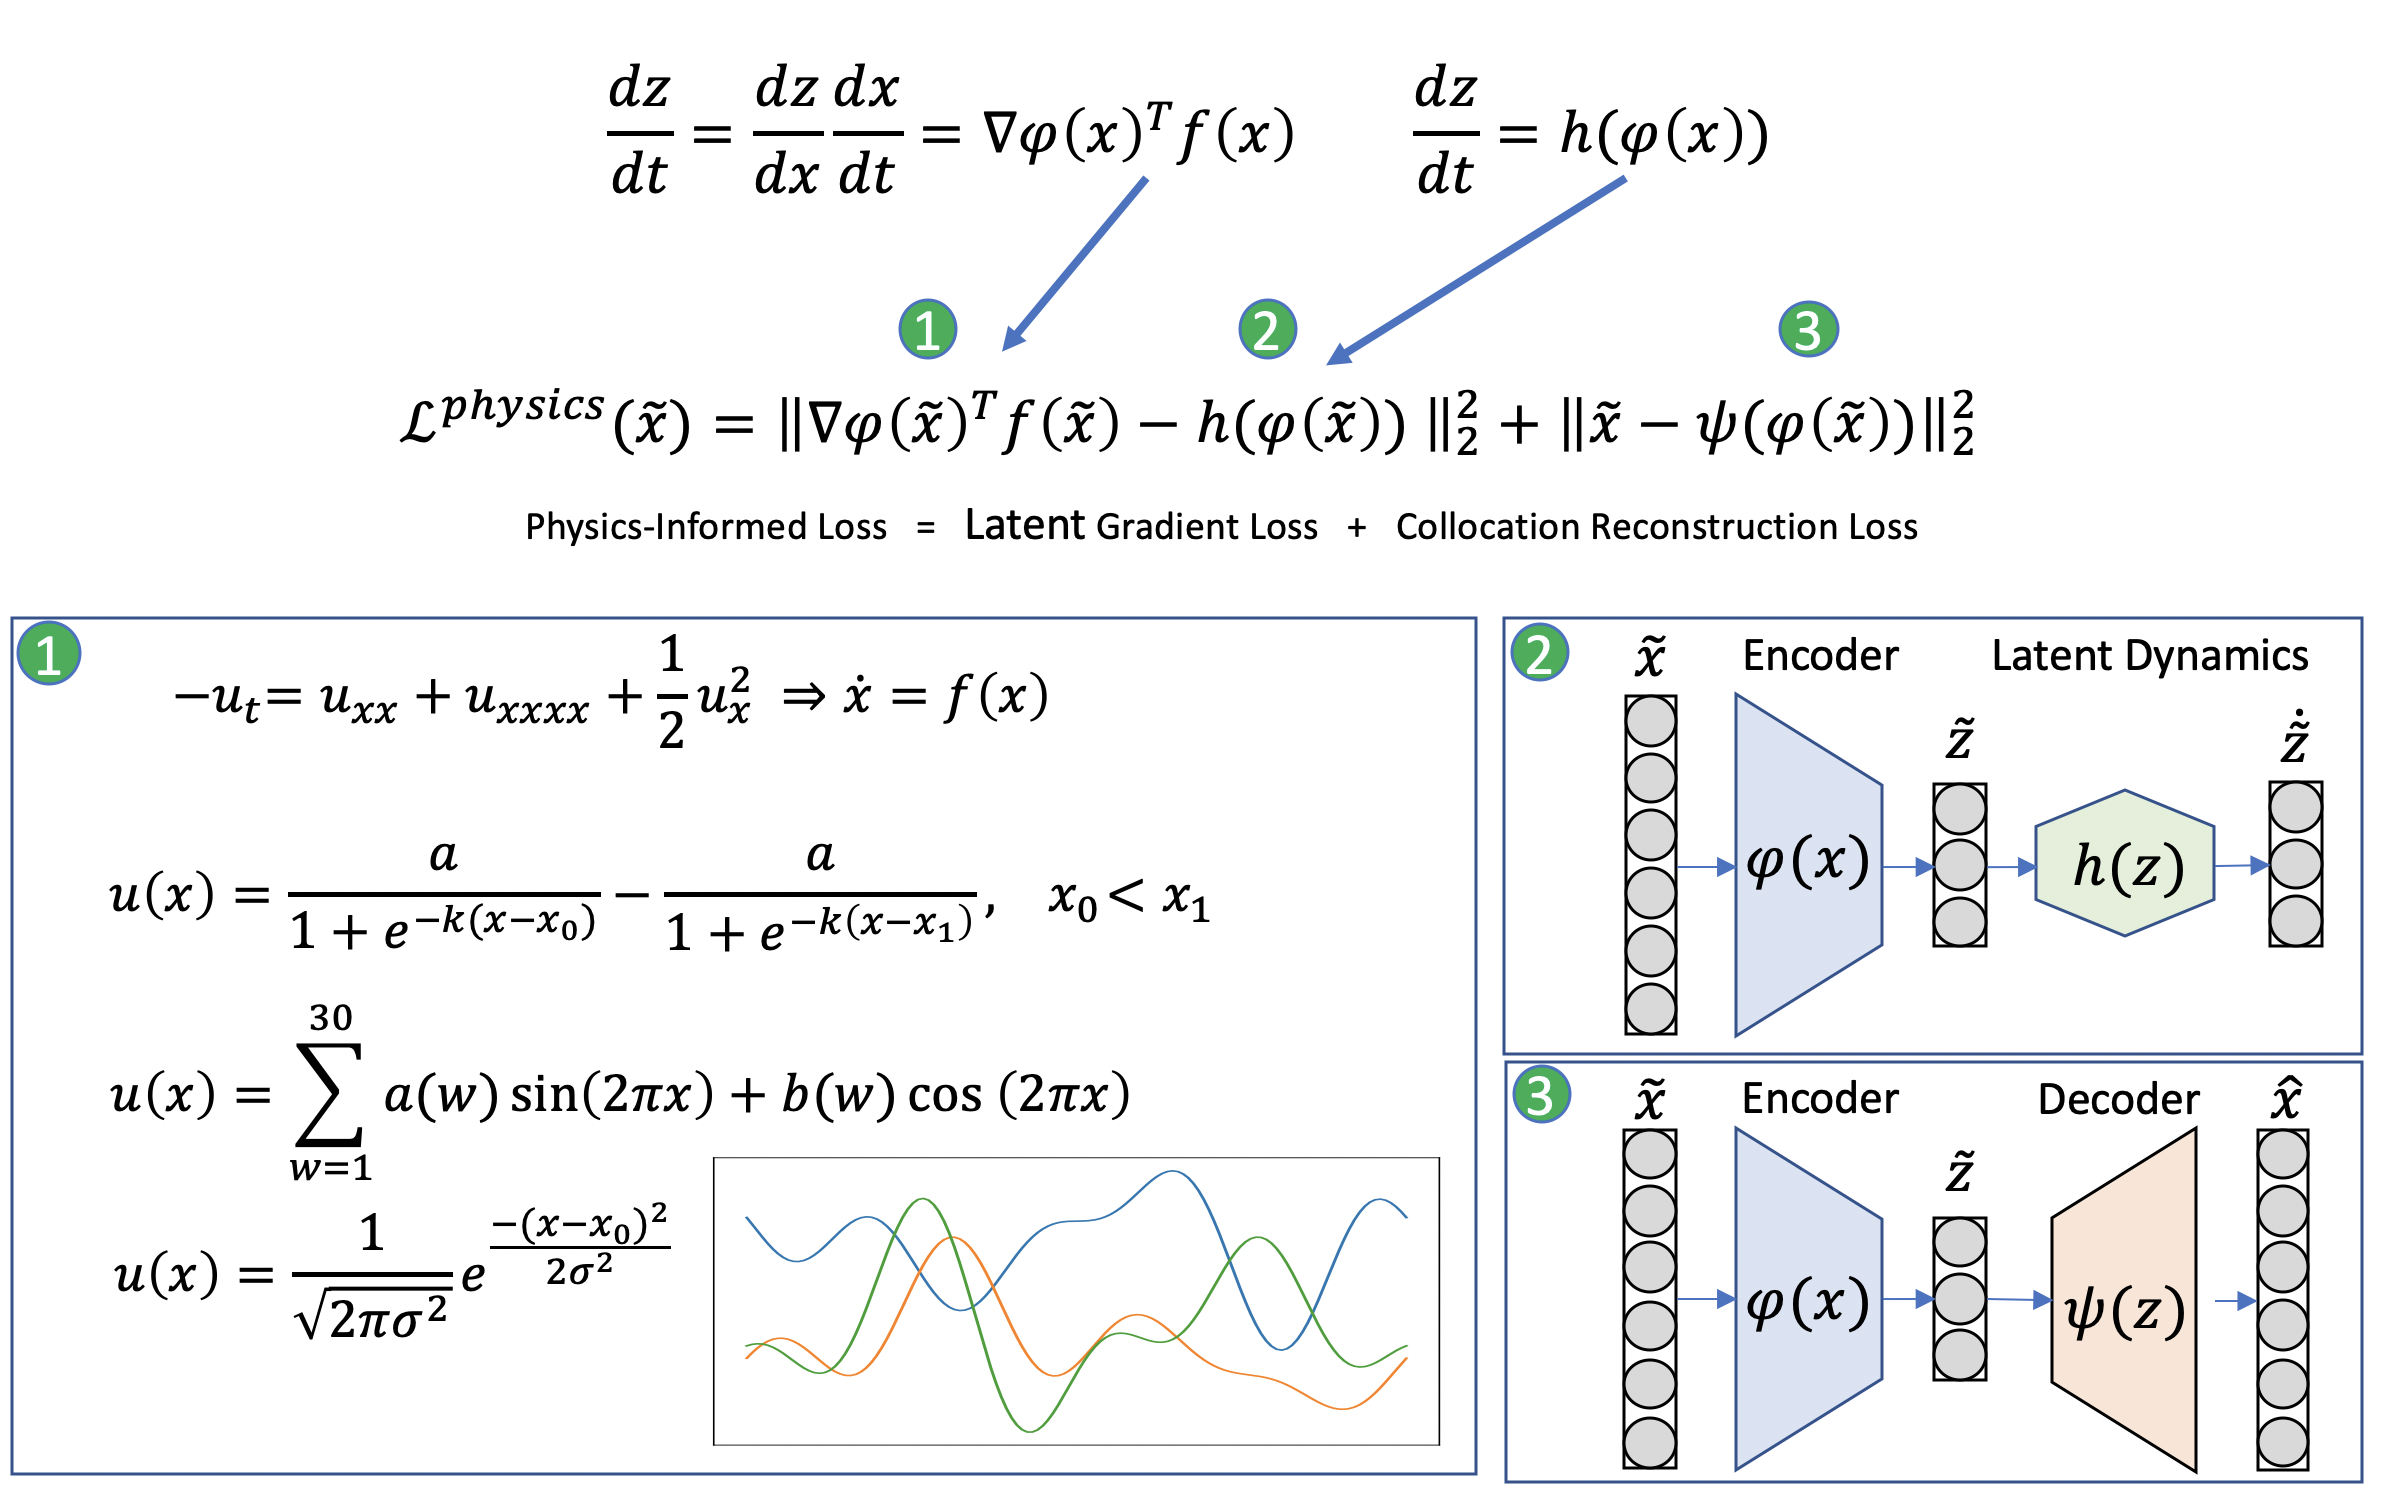
\includegraphics[width=\textwidth]{Figures/collocations_5.png}}
\end{frame}



\begin{frame}{Results: Extrapolation to Unknown Regions}
% 1) We show that network can indeed interpolate between collocations. Moreover, it can fill the whole unknown regimes of behavior. (Duffing example with explanation)
Duffing Oscillator on a low-dimensional (2D) manifold:
\begin{equation}
    \label{eq:duffing_definition}
    \begin{split}
    \frac{dz_1}{dt} & = z_2 \\ 
    \frac{dz_2}{dt} & = z_1 - z_1^3
    \end{split}
\end{equation}

Projection to a high-dimensional (128) space:
\begin{equation}
    \label{eq:duffing_true_decoder}
    \bd{x} := \mathcal{A}(\bd{z}) = A\bd{z}^3, \quad A \in \mathbb{R}^{128 \times 2}, \quad A_{ij} \sim_{i.i.d.} \mathcal{N}(0, 1)
\end{equation}
\uncover<2->{
\begin{figure}
	\centering
	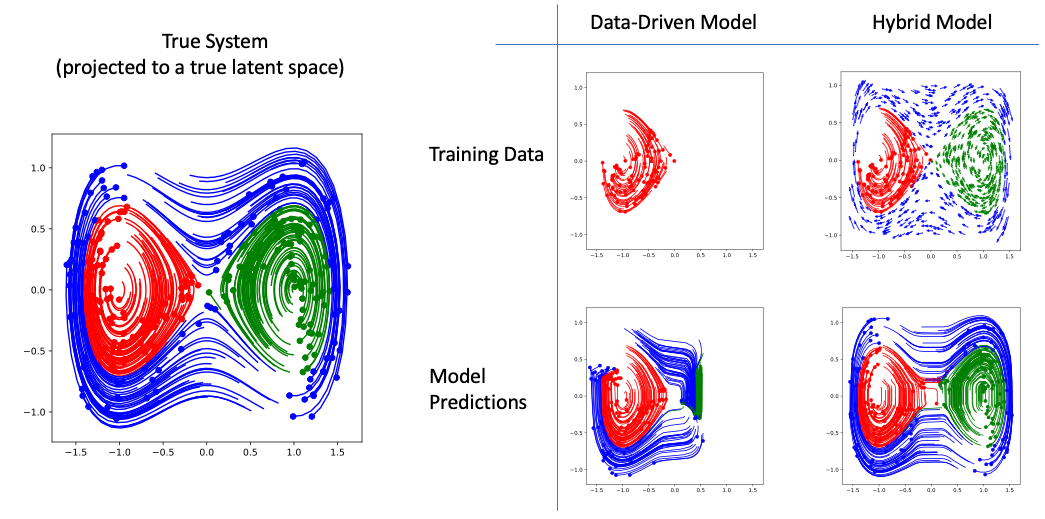
\includegraphics[width=0.8\textwidth]{Figures/duff_results.png}
\end{figure}
}
\end{frame}

\begin{frame}{Results: Stable Long-Term Predictions}
\begin{figure}
	\begin{subfigure}[b]{0.3\textwidth}
		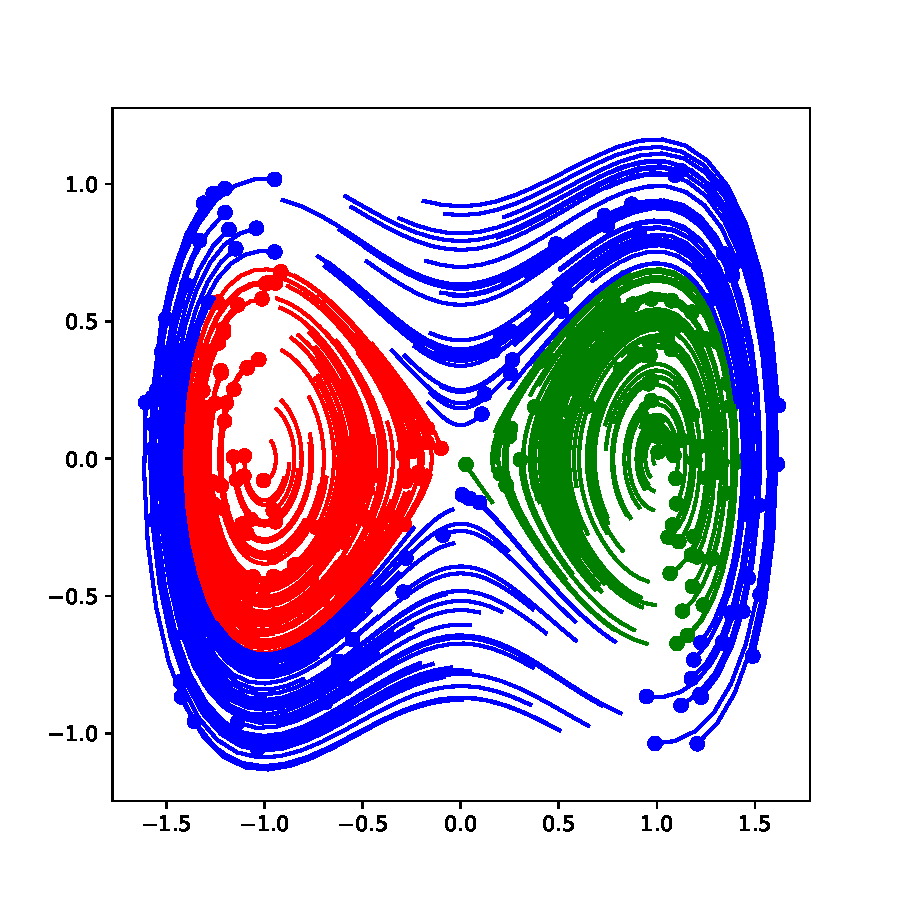
\includegraphics[width=\textwidth]{Figures/duff_full_train.pdf}
	\end{subfigure}%
	\begin{subfigure}[b]{0.7\textwidth}
		\centering
		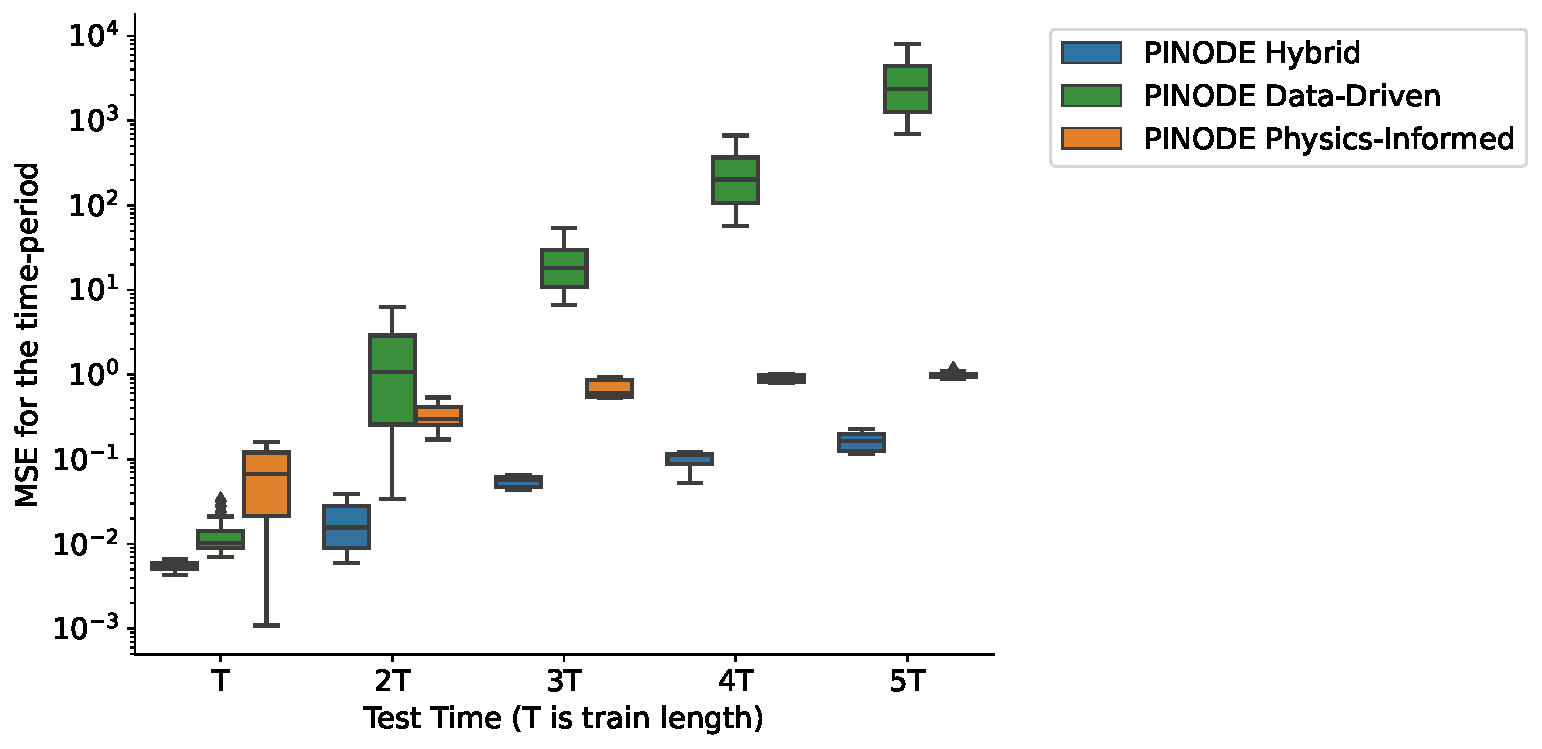
\includegraphics[width=0.7\textwidth]{Figures/duffing_periods.pdf}
	\end{subfigure}
\end{figure}
\uncover<2->{
\begin{figure}
	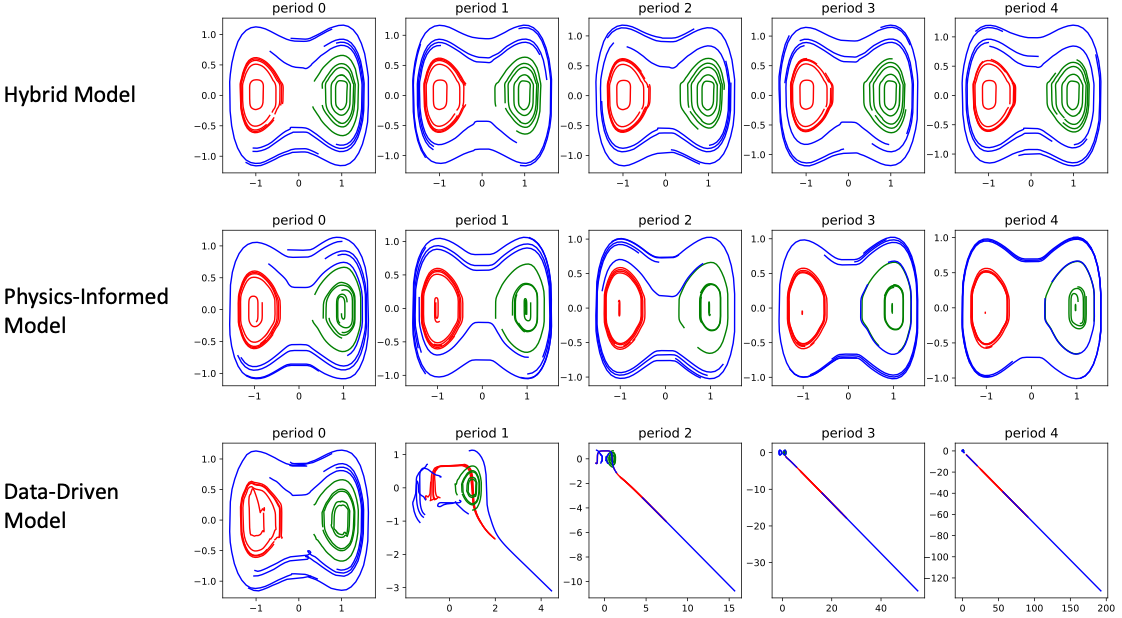
\includegraphics[width=0.7\textwidth]{Figures/duffing_periods_examples.png}
\end{figure}
}
\end{frame}

\begin{frame}{Results: Burgers' Equation}
Burgers' Equation:
\begin{equation}
	\begin{split}
		& u_t  + uu_x = \nu u_{xx} \\
	    & u(-\pi, t) = u(\pi, t),\quad \forall t \in [0, T]
	\end{split}
\end{equation}
\uncover<2->{
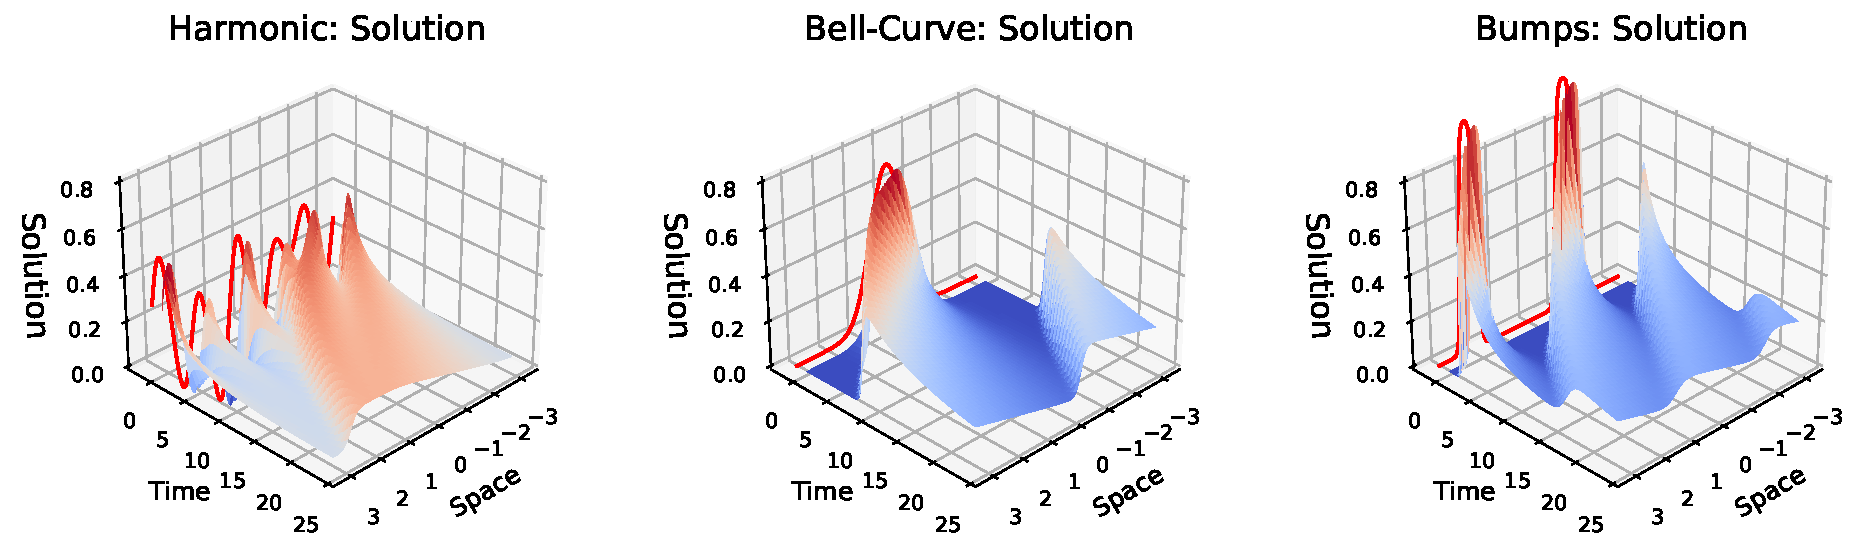
\includegraphics[width=\textwidth]{Figures/burgers_examples_of_ics.pdf}
}
\uncover<3->{
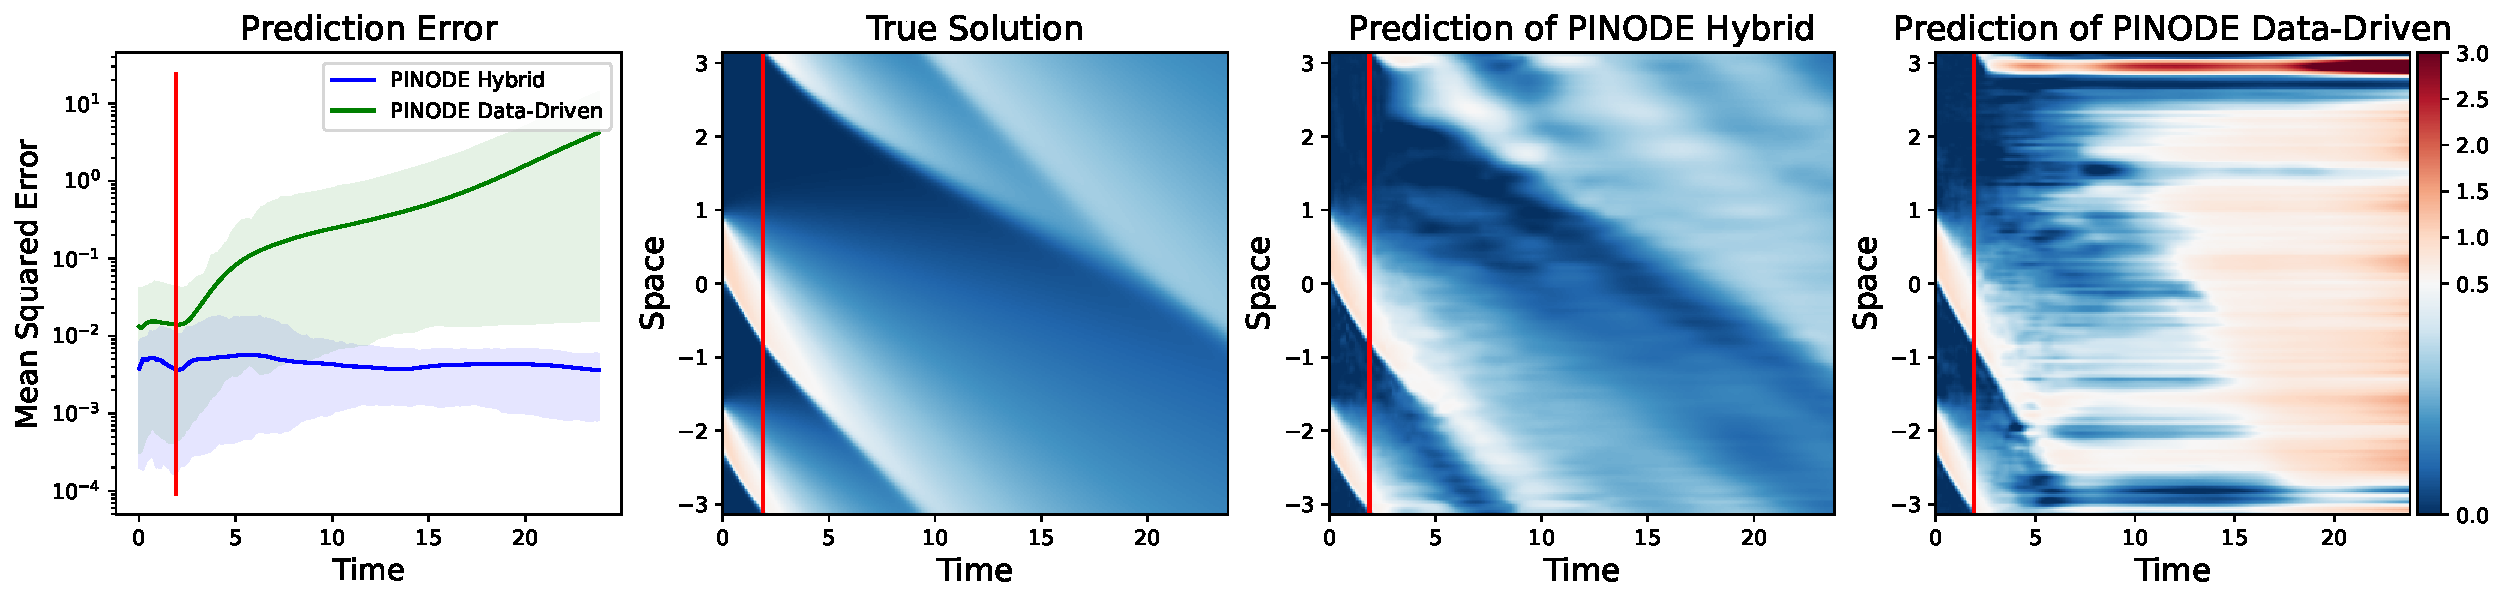
\includegraphics[width=\textwidth]{Figures/example_burgers.pdf}
}

\end{frame}

\begin{frame}{Results: Learning From Collocations}
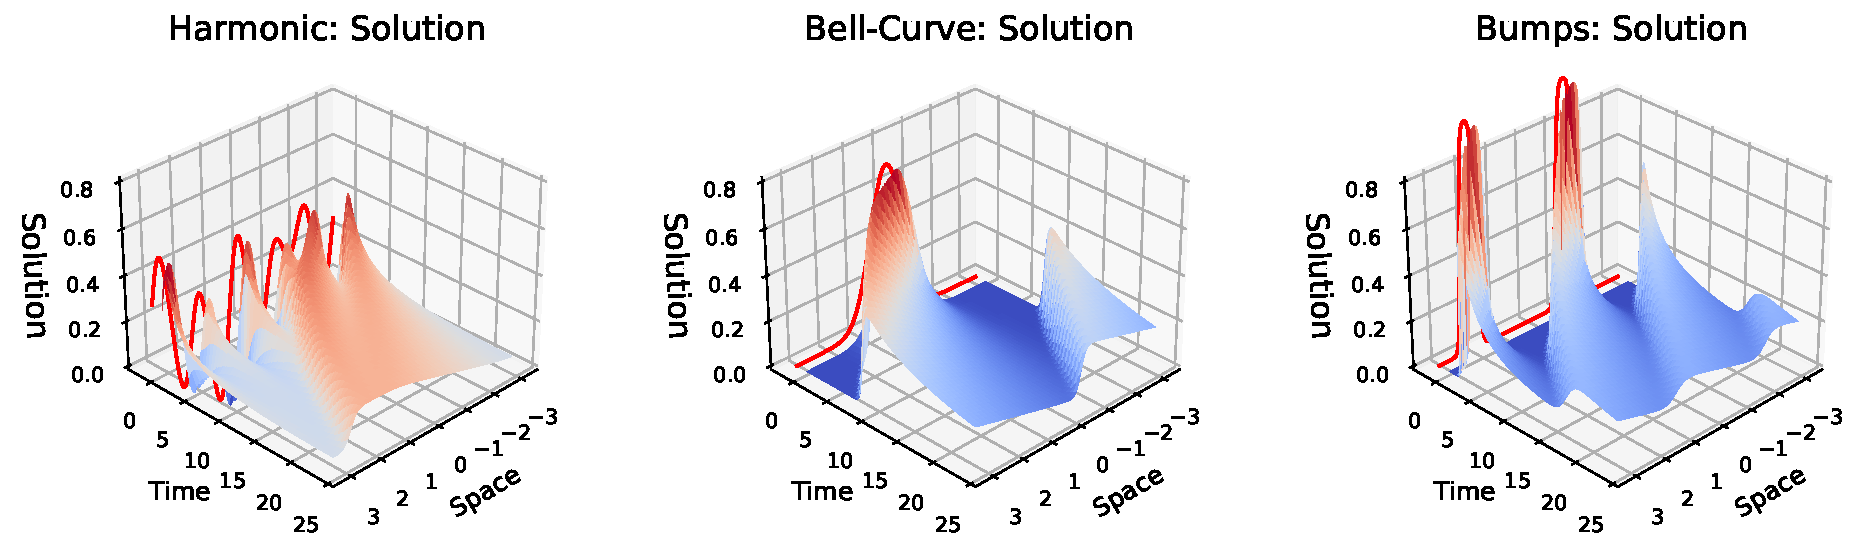
\includegraphics[width=\textwidth]{Figures/burgers_examples_of_ics.pdf}
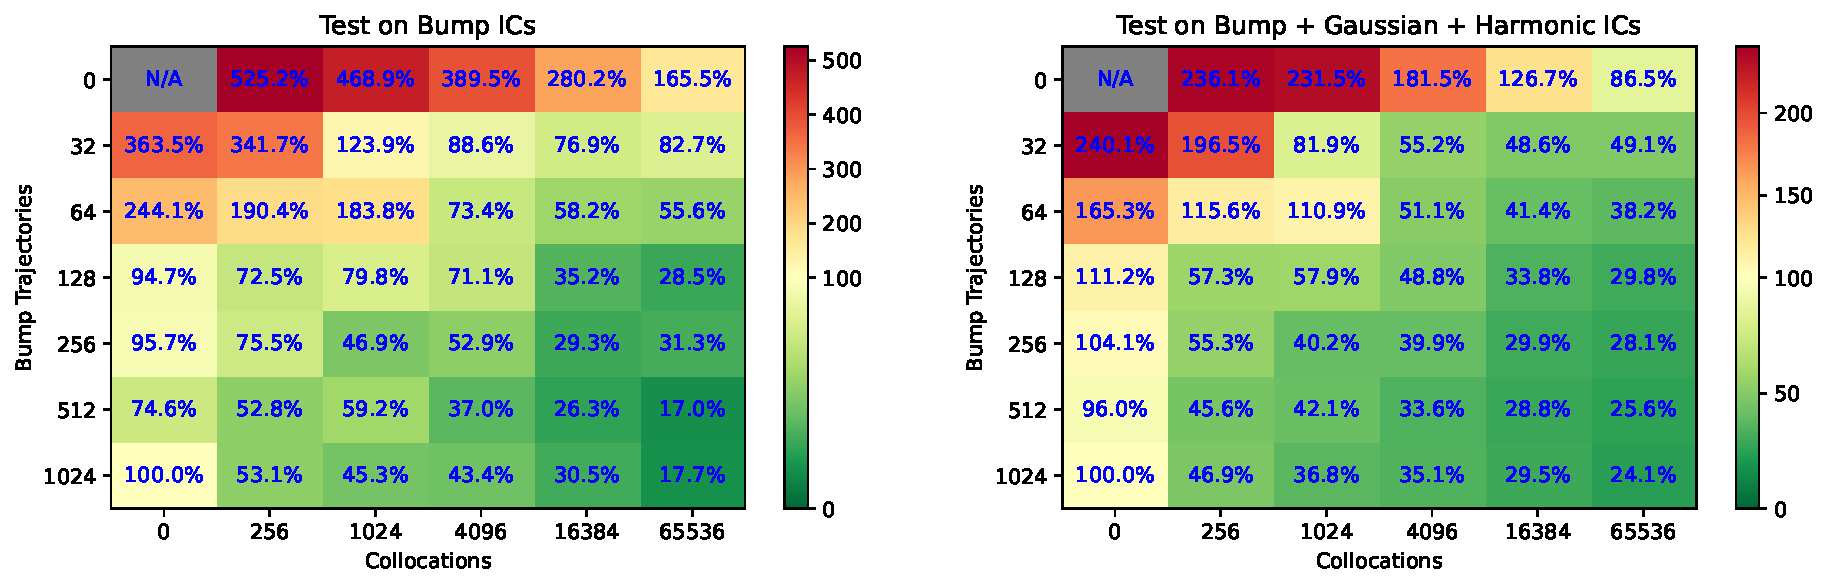
\includegraphics[width=\textwidth]{Figures/data_vs_collocations.pdf}
\end{frame}

\begin{frame}{Discussion and Limitations}
We showed that:
\begin{itemize}
	\item Physics-informed loss improves accuracy and forecasting stability of ROMs
	\item Collocations can supplement data to improve model's performance for unseen initial conditions.
\end{itemize}
\vspace{2em}
Limitations:
\begin{itemize}
	\item Optimal choice of collocations is problem-specific
	\item Need a lot of collocations
	\begin{itemize}
		\item \textit{Could} be possible to overcome with smarter sampling techniques
	\end{itemize}
\end{itemize}
\end{frame}

\section{Single pixel imaging of spatio-temporal flows using differentiable latent dynamics}

\begin{frame}{Single-Pixel Imaging}
%1) Now we switch gears to show you an application to single-pixel imaging
%2) It shows how powerful these differentiable reduced-order models can be in applications besides forecasting and motivate the need to improve those.
%3) SPI setup is a single-pixel camera with mirror array… 
\begin{figure}
	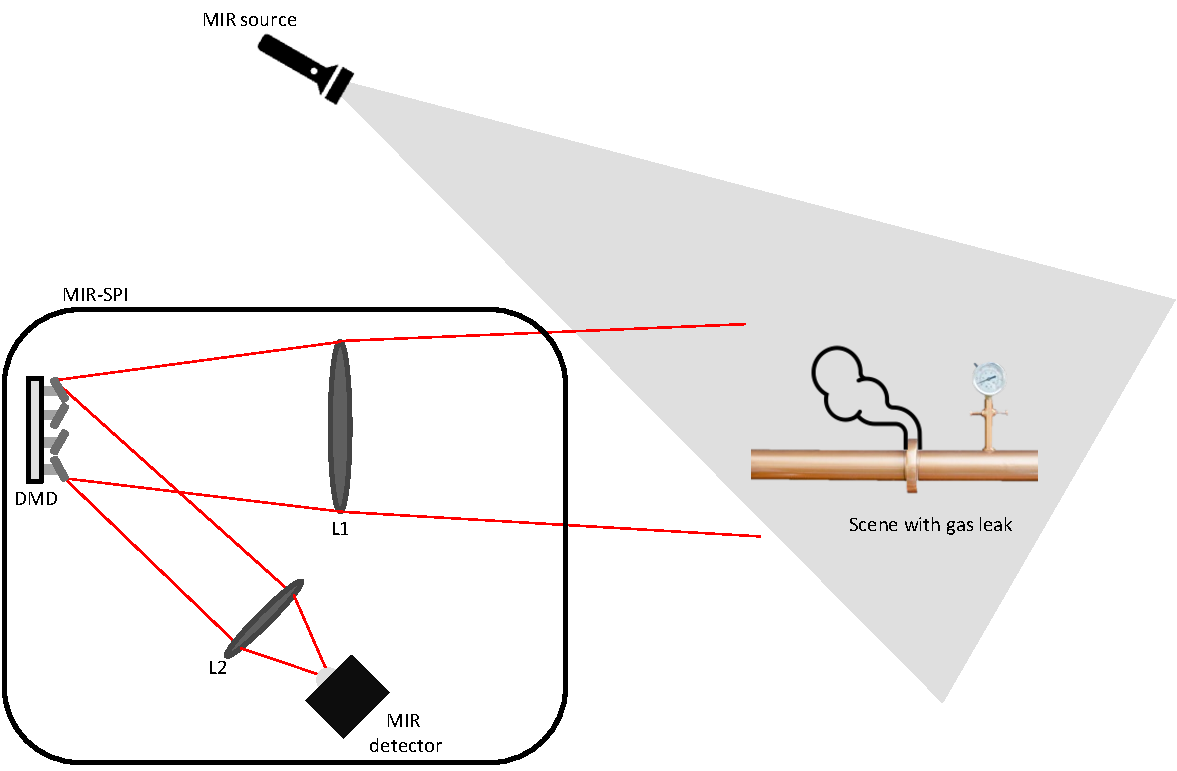
\includegraphics[width=\textwidth]{Figures/SPI_setup.pdf}
\end{figure}
\end{frame}


\begin{frame}{Single-Pixel Imaging}
	% This is how SPI setup translates into Math
	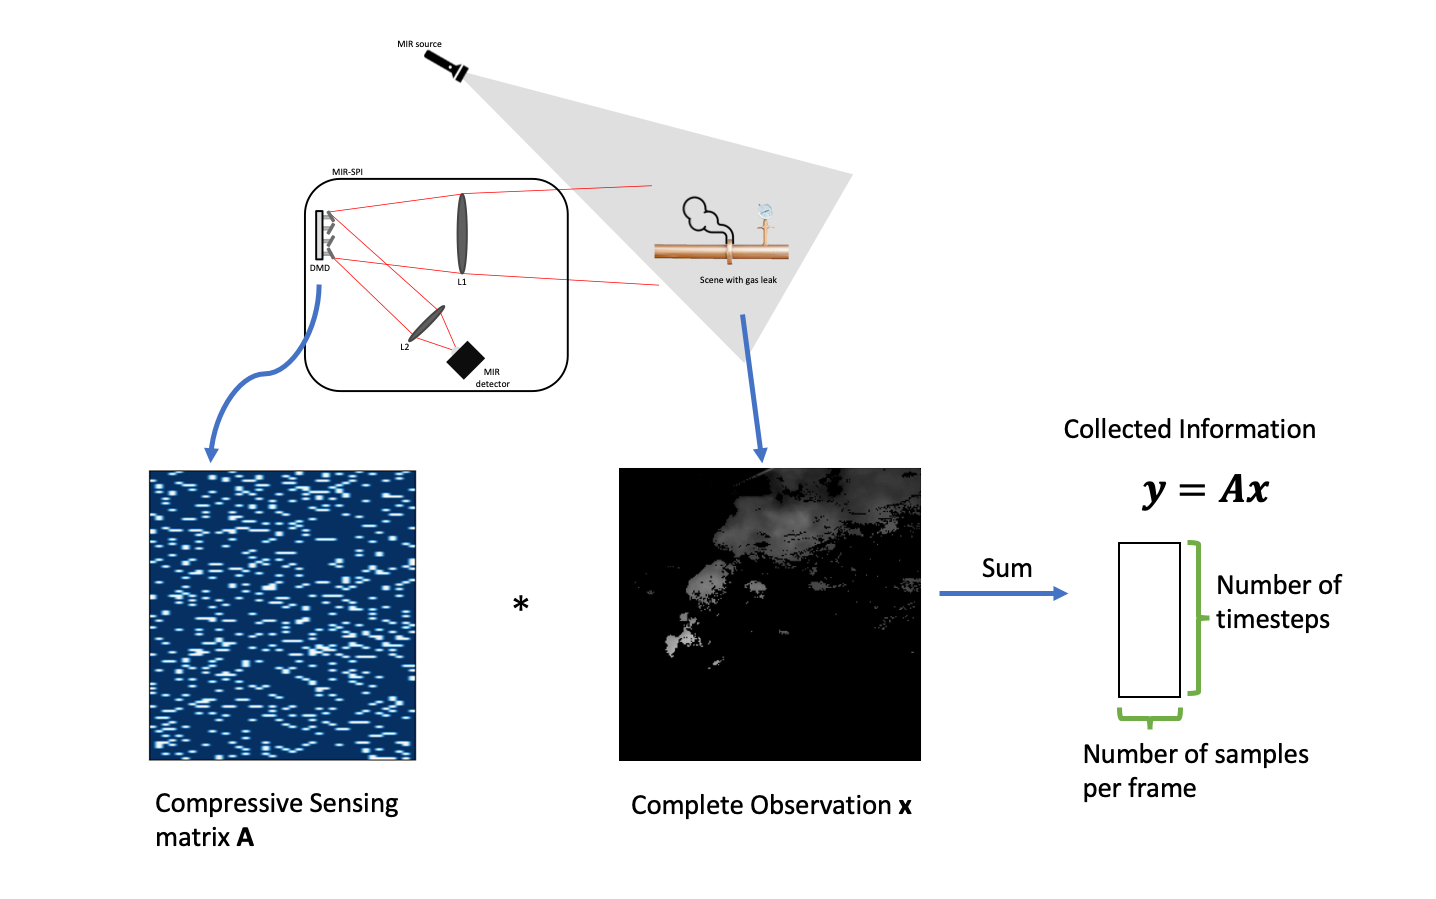
\includegraphics[width=\textwidth]{Figures/spi_math.png}
\end{frame}


\begin{frame}{Compressive Sensing with Reduced-Order Models}
	%1) We introduce a ROM as a relaxation of a PDE-constrained compressive sensing.
	%2) We search in the latent space of a ROM for the right trajectory that matches both the ROMs predictions and the compressive-sensing observations
	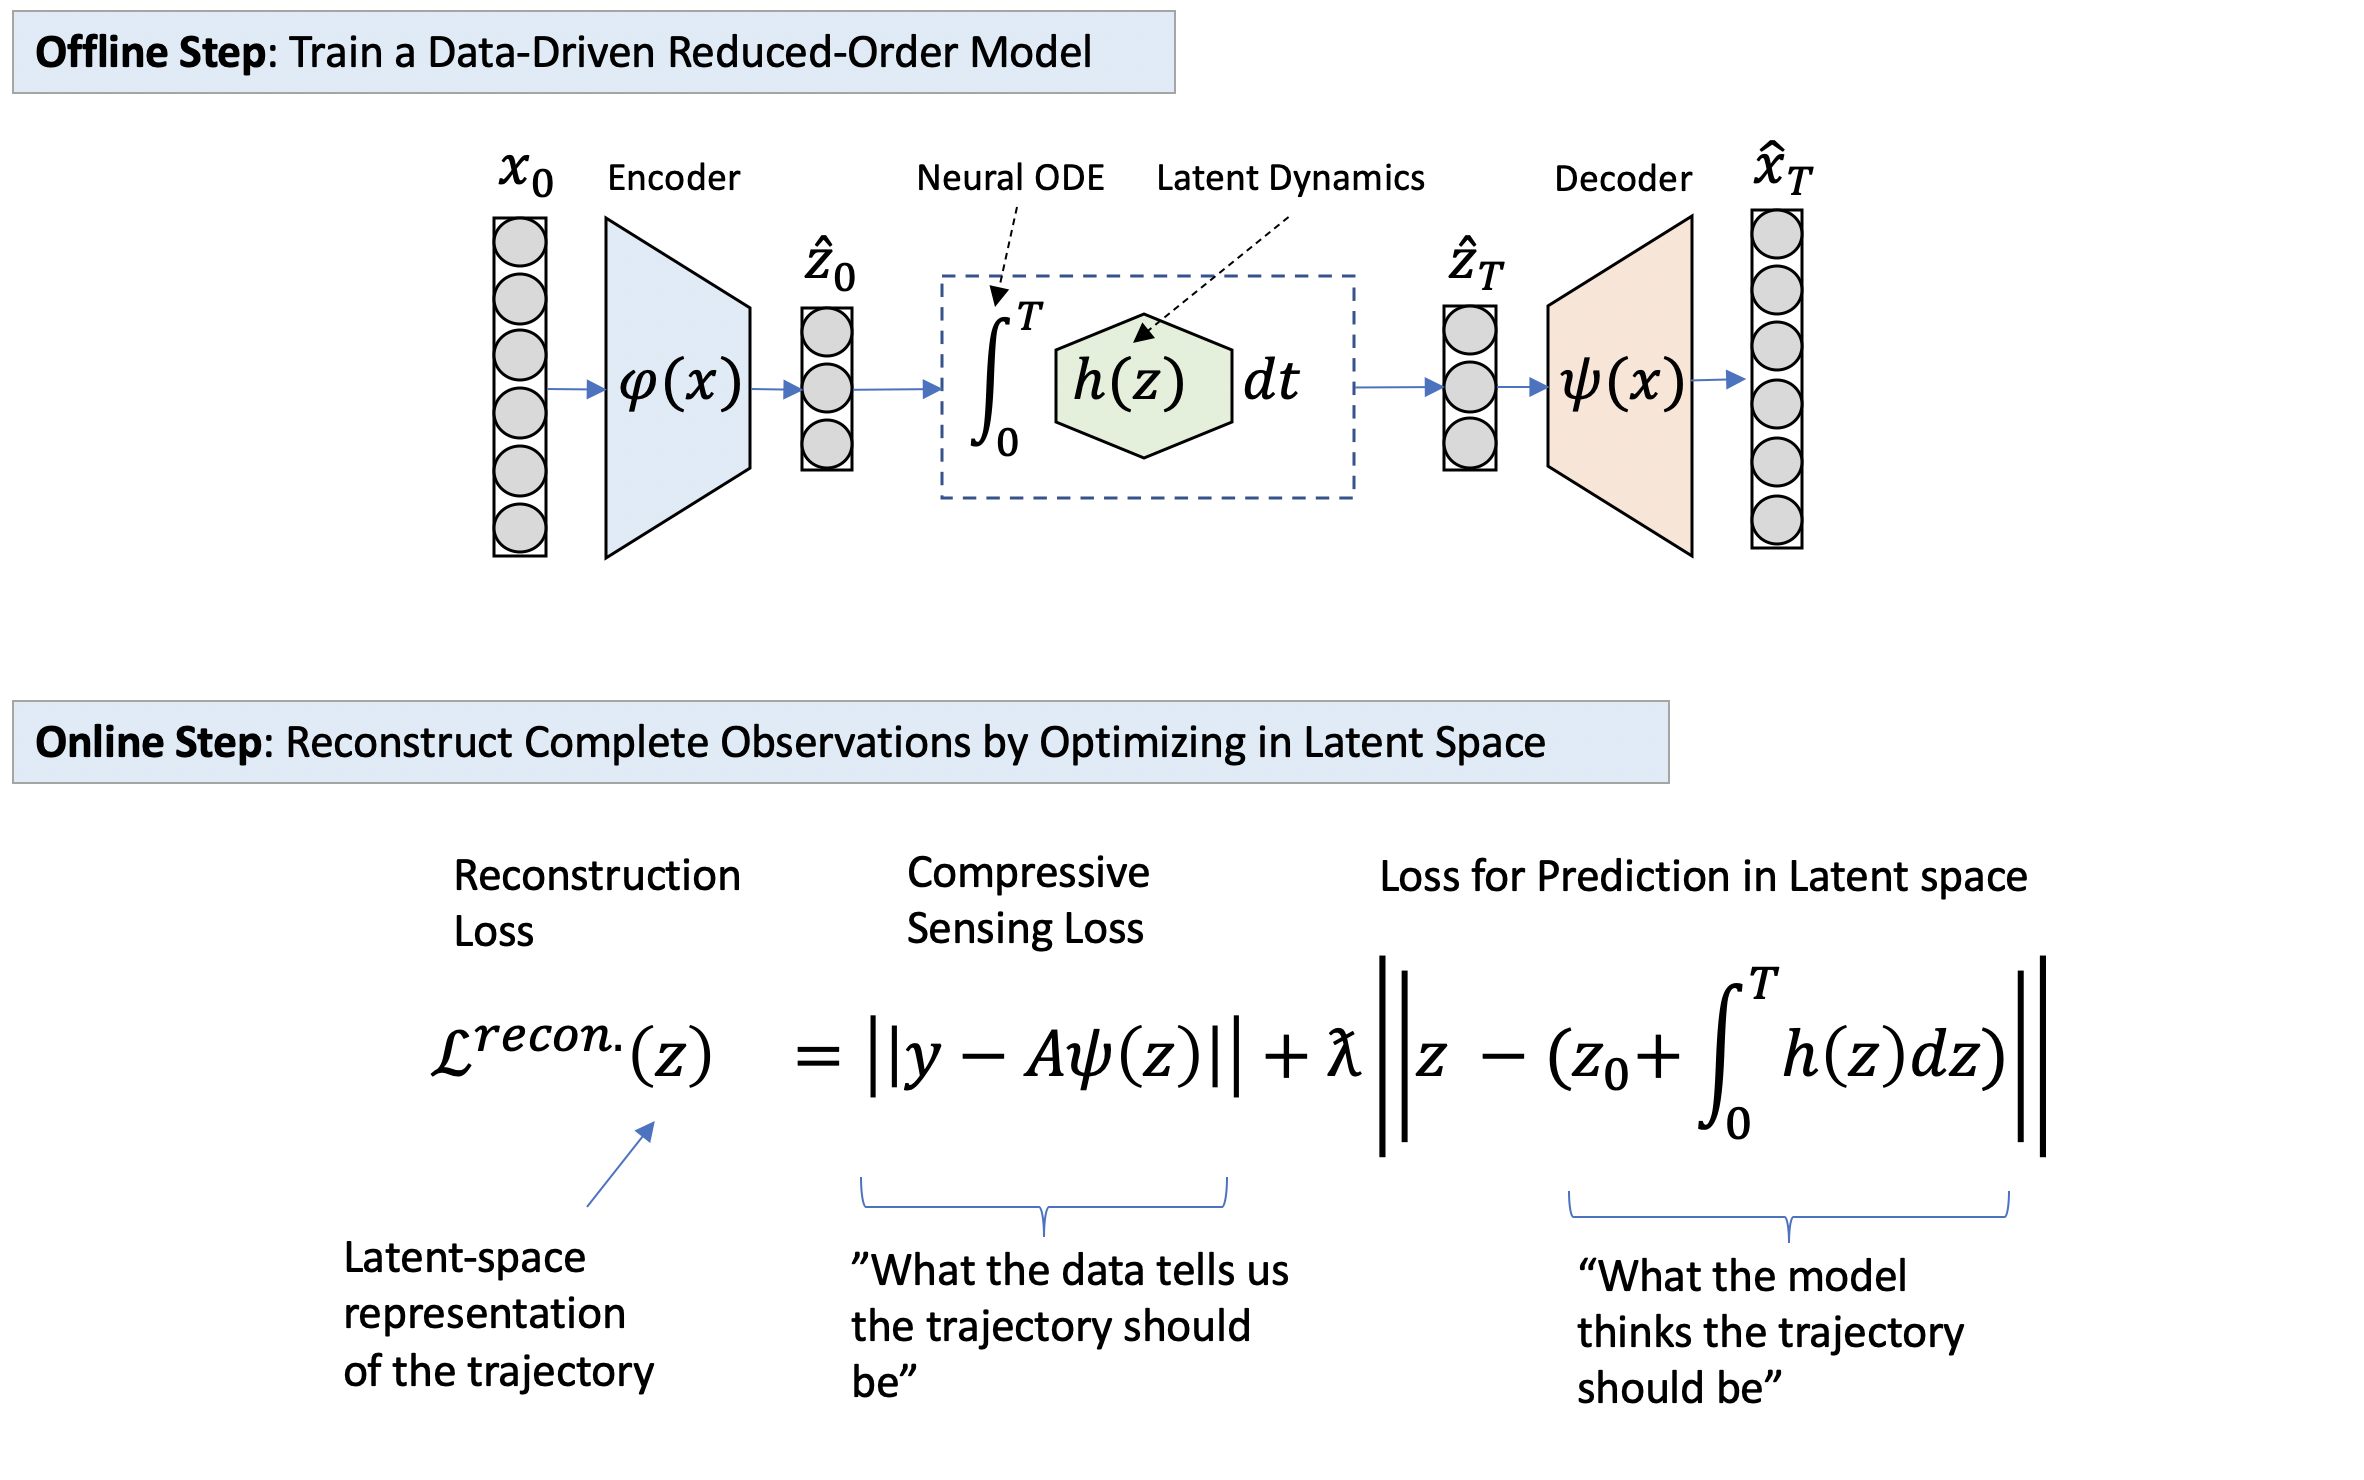
\includegraphics[width=\textwidth]{Figures/cs_schematics.png}
\end{frame}

\begin{frame}{Results: Burger's Equation}
	When we capture 32 samples per frame:
	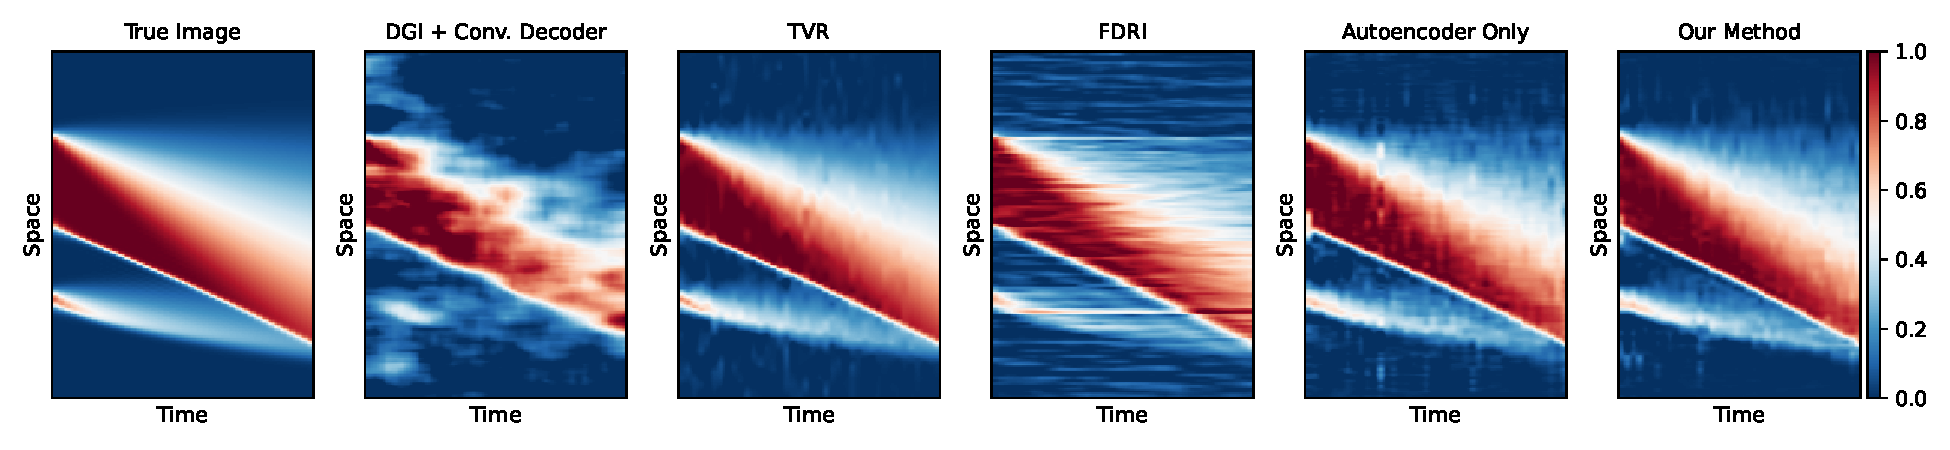
\includegraphics[width=\textwidth]{Figures/cs_burgers_comparison_32.pdf}
\end{frame}

\begin{frame}{Results: Burger's Equation}
	When we capture 32 samples per frame:
	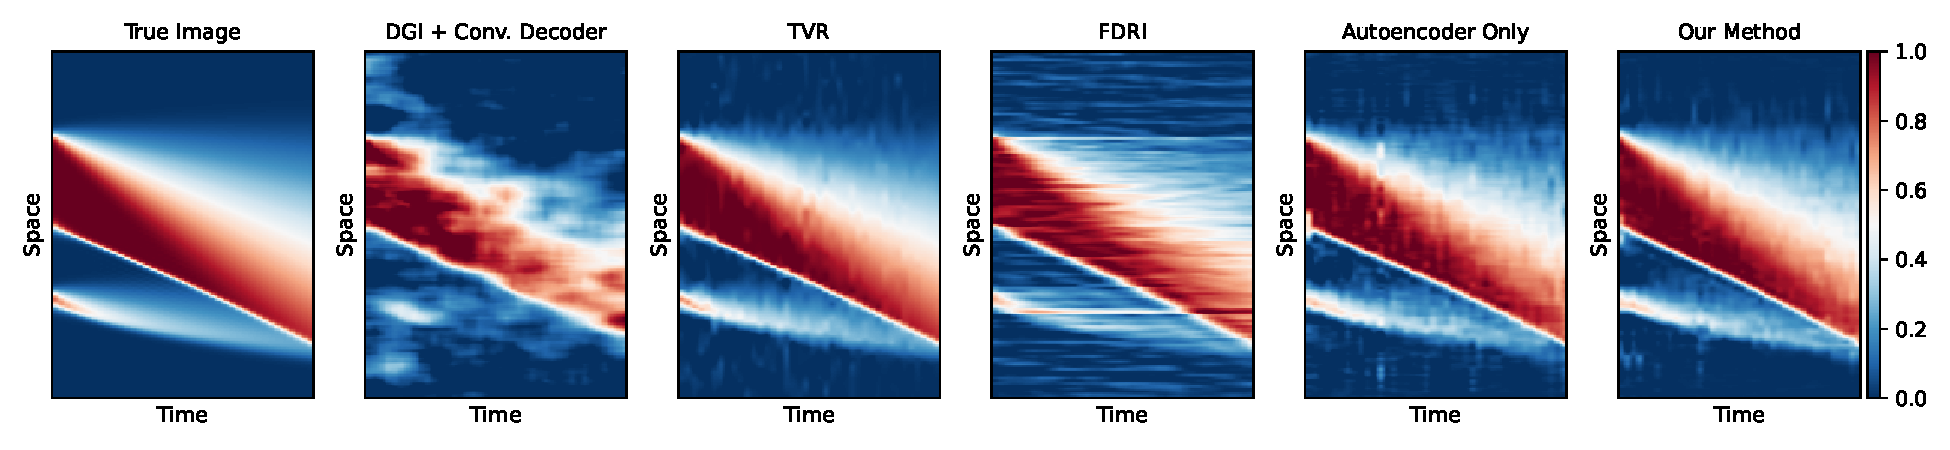
\includegraphics[width=\textwidth]{Figures/cs_burgers_comparison_32.pdf}
	
	When we capture 2 samples per frame:
	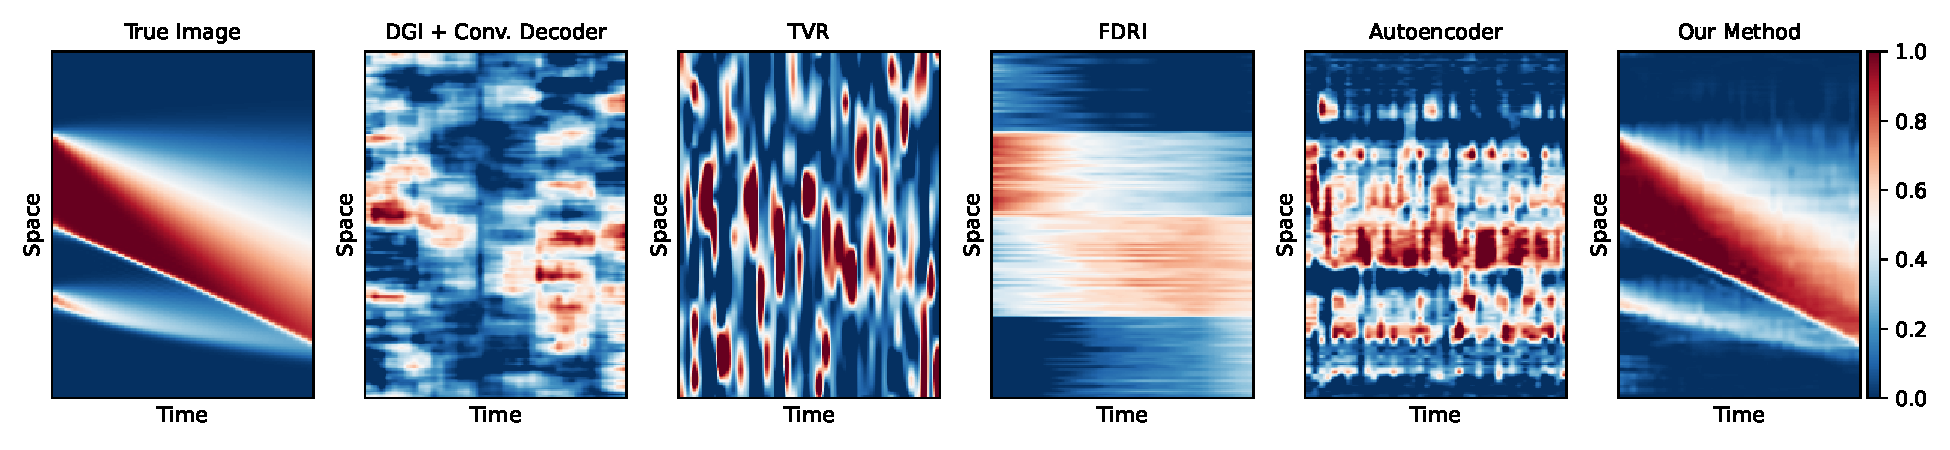
\includegraphics[width=\textwidth]{Figures/cs_burgers_comparison_2.pdf}
\end{frame}

\begin{frame}{Results: Burger's Equation}
	Aggregated results
\end{frame}

\begin{frame}{Results: Interpretation}
	
\end{frame}

\begin{frame}{Results: Kolmogorov Flow OR Real Example}
\end{frame}

\begin{frame}{Conclusion}
	Results on Burgers
	Maybe results on a harder problem
\end{frame}

\appendix
\section{Appendix: $\mathcal{MSR}3$}
\begin{frame}{Designing an Algorithm}
	$G_{\nu,\eta}$ encodes both gradient of a Lagrangian (lines 1-2) and the complementarity condition (line 3):
	\eq{
		G_{\nu,\eta}((\beta,\gamma,v),(\tbeta,\tgamma)) := \begin{bmatrix}
			\nabla_\beta \LL(\beta, \gamma) + \eta(\beta-\tbeta) \\
			\nabla_\gamma \LL(\beta, \gamma) + \eta(\gamma-\tgamma) - v\\
			v \bigodot \gamma - \mu\textbf{1}
		\end{bmatrix}
	}
	We apply Newton method to $G$ while geometrically decreasing $\mu$. \\
\textbf{Lemma:} For every $(\mu,\eta) \in \R_+\times\R_{++}$,
\eq{
	&(\hat\beta,\hat\gamma) = \argmin_{(\beta,\gamma)}\LL_{\eta,\mu}((\beta, \gamma),(\tbeta, \tgamma)) \\
	& \iff \\
	& \exists \hat{v} \in \R_{+}^q \text{ s.t. } G_{\nu,\eta}((\beta,\gamma,\hat{v}),(\tbeta,\tgamma)) = 0
}
If $\mu > 0$, then $\hat{v} = -\nabla\phi_\mu(\hat{\gamma})$, and if $\mu = 0$, then $\hat{v}$ is the unique KKT multiplier associated with the constraint $0 \leq \gamma$.
\end{frame}

\begin{frame}{$\ouralgo$-fast Algorithm}
\label{appendix:pseudocode}
\begin{algorithm}[H]
\SetAlgoLined
$\texttt{progress}\leftarrow \textbf{True}$; \quad \texttt{iter = 0}; \\
$\beta^+, \tbeta^+\leftarrow\beta_0$; 
\quad $\gamma^+, \tgamma^+\leftarrow\gamma_0$;  
\quad $v^+ \leftarrow 1 \in \R^q$; 
\quad  $\mu \leftarrow \frac{{v^+}^T\gamma^+}{10 q}$\\
 \While{\texttt{iter} $<$ \texttt{max\_iter}  \ and \ $\|G_\mu(\beta^+, \gamma^+, v^+)\|$ $>$ \texttt{tol}   \ and  \ \texttt{progress} \\}{
    $\beta \leftarrow \beta^+$; \quad $\gamma \leftarrow \gamma^+$; \quad $\tbeta \leftarrow \tbeta^+$; \quad $\tgamma \leftarrow \tgamma^+$ \\
%    $A \leftarrow \nbla G_\mu((\beta, \gamma, v), (\tbeta, \tgamma))$\\
  %  $b \leftarrow G_\mu((\beta, \gamma, v), (\tbeta, \tgamma))$\\
    $[dv, d\beta, d\gamma] \leftarrow  \nabla G_\mu((\beta, \gamma, v), (\tbeta, \tgamma))^{-1}  G_\mu((\beta, \gamma, v), (\tbeta, \tgamma))$
    $\alpha \leftarrow 0.99\times\min\left(1, -\frac{\gamma_i}{d\gamma_i}, \forall i :\ d\gamma_i < 0\right)$\\
    $\beta^+ \leftarrow \beta + \alpha d\beta$; \quad $\gamma^+ = \gamma + \alpha d\gamma$; \quad  $v^+ \leftarrow v + \alpha dv$\\
    \lIf{$\|\gamma^+\odot v^+ - q^{-1}{\gamma^+}^Tv^+ \mathbf{1}\| > 0.5q^{-1}{v^+}^T\gamma^+$}{continue}
    \Else{ 
        $\tbeta^+ = \prox_{\alpha R}(\beta^+)$;
        \    $\tgamma^+ = \prox_{\alpha R + \delta_{\R_+}}(\gamma^+)$; 
        \    $\mu = \frac{1}{10}\frac{{v^+}^T\gamma^+}{q}$
    }
%	\tcp*[h]{Keep iterating until convergence} \\
    \texttt{progress} = ($\|\beta^+ - \beta\| \geq \text{tol}$ or $\|\gamma^+ - \gamma\|  \geq \text{tol}$ or $\|\tbeta^+ - \tbeta\| \geq \text{tol}$ or $\|\tgamma^+ - \tgamma\| \geq \text{tol}$)\\
    \texttt{iter += 1}
 }
 \Return{$\tbeta^+$, $\tgamma^+$}
\end{algorithm}

\end{frame}

\begin{frame}[noframenumbering,plain,allowframebreaks]{References}
    \printbibliography[heading=none]
\end{frame}

\end{document}